\documentclass[]{article}
\usepackage[english]{babel}
\usepackage{amsmath, amsfonts, amssymb, dsfont}
\usepackage{float}
\usepackage{fancyhdr}
\usepackage{fontawesome5}
\usepackage{mathrsfs}
\usepackage{amsmath}
\allowdisplaybreaks 
\usepackage{arydshln} 
\usepackage{tikz}
\usetikzlibrary{automata, positioning}
\usepackage[T1]{fontenc}
\usepackage{lmodern}
\usepackage{listings}
\usepackage{inconsolata}
\usepackage{upquote}    
\usepackage{mathtools}
\definecolor{rstudioBG}{RGB}{250,250,250}
\definecolor{rstudioFrame}{RGB}{220,220,220}
\definecolor{rstudioBlue}{RGB}{0,92,197}  
\definecolor{rstudioGreen}{RGB}{0,128,0}   
\definecolor{rstudioRed}{RGB}{163,21,21} 
\definecolor{rstudioNum}{RGB}{128,0,128}  

\lstdefinelanguage{R}{
  alsoletter={._},
  morekeywords={if,else,repeat,while,function,for,in,next,break,TRUE,FALSE,NA,NaN,Inf,NULL},
  morekeywords={[2]library,require,data,plot,ggplot,geom_point,geom_line,aes,
               summary,lm,glm,anova,predict,confint,print,cat,read.csv,head,
               dplyr,mutate,select,filter,arrange,group_by,summarise,as.factor,
               factor,as.numeric,as.character,seq,rep,mean,median,sd,var,cor},
  sensitive=true
}

\lstdefinestyle{RStudio}{
  language=R,
  basicstyle=\ttfamily\footnotesize,
  backgroundcolor=\color{rstudioBG},
  frame=single,
  framerule=0.4pt,
  rulecolor=\color{rstudioFrame},
  framesep=6pt,
  numbers=left,
  numberstyle=\tiny\color{gray},
  numbersep=8pt,
  showstringspaces=false,
  breaklines=true,
  columns=fullflexible,
  keepspaces=true,
  keywordstyle=\color{rstudioBlue}\bfseries,     
  keywordstyle={[2]\color{rstudioBlue}},       
  commentstyle=\itshape\color{rstudioGreen},
  stringstyle=\color{rstudioRed},
  literate=
    *{0}{{{\color{rstudioNum}0}}}{1}
     {1}{{{\color{rstudioNum}1}}}{1}
     {2}{{{\color{rstudioNum}2}}}{1}
     {3}{{{\color{rstudioNum}3}}}{1}
     {4}{{{\color{rstudioNum}4}}}{1}
     {5}{{{\color{rstudioNum}5}}}{1}
     {6}{{{\color{rstudioNum}6}}}{1}
     {7}{{{\color{rstudioNum}7}}}{1}
     {8}{{{\color{rstudioNum}8}}}{1}
     {9}{{{\color{rstudioNum}9}}}{1},
}

\lstset{style=RStudio}


\usepackage{hyperref}
\usepackage[utf8]{inputenc}

\usepackage{graphicx, adjustbox, float, xcolor}

\usepackage{tikz, pgfplots}
\pgfplotsset{compat=1.17}
\usepackage{placeins}
\usetikzlibrary{arrows.meta, automata, positioning, decorations.pathreplacing, decorations.markings}
\newcommand{\interior}[1]{%
  {\kern0pt#1}^{\mathrm{o}}%
}

\usepackage{booktabs, enumitem, caption}
\usepackage{amsmath}
\usepackage{amssymb}
\usepackage{gensymb}


\usepackage[a4paper,
  includehead,includefoot,
  top=5mm,          
  headheight=15pt,  
  headsep=1pt,       
  bottom=20mm,left=40mm,right=40mm
]{geometry}

\pagestyle{fancy}



\lhead{Ben Vickers - 304024}
\rhead{Linear Statistical Models Worksheet 1}
\setlength{\headsep}{0.4cm}
\usepackage{titling}
\setlength{\droptitle}{-70pt}   

\title{\textbf{Linear Statistical Models Worksheet 1}}
\author{Ben Vickers - 304024}
\date{\textbf{Due: 19:59, Thursday 20 November 2025}}

\begin{document}
	\maketitle
   
\noindent The dataset \textbf{satgpa} contains the academic records of 1000 students at an unnamed US college. It contains the following information of each student: first year grade point average at college (variable \textbf{fy\_gpa}), their verbal SAT percentile (variable \textbf{sat\_v}), their maths SAT percentile (variable \textbf{sat\_m}), the total of their SAT percentiles (variable \textbf{sat\_sum}), their high school grade point average (variable \textbf{hs\_gpa}) and their sexes (variable \textbf{sex}, 1= male, 2= female).

\begin{enumerate}
\item Use a multiple regression model to explore the relationship between
a person’s first year grade point average, their SAT percentile, and their high
school grade point average. Comment on the predictive power of the model.
\end{enumerate}


\noindent \textbf{SOLUTION:}\newline

\noindent We aim to explore whether a student's first year performance at College (University) can be predicted based on their high school SAT and GPA statistics. We begin by fitting the model:

\[
\textit{fy\_gpa}_i = \beta_0 + \beta_1 \textit{sat\_sum}_i + \beta_2  \textit{hs\_gpa}_i + \varepsilon_i \quad;\quad \varepsilon_i\overset{\text{iid}}{\sim}\mathcal{N}(0,\sigma^2)
\]

\noindent We can do this in \textsf{R}:

\begin{lstlisting}[language=R]
md <- lm(fy_gpa ~ sat_sum + hs_gpa, data = satgpa)
\end{lstlisting}

\noindent We then aim to perform an F-test on the predictive power of the model:

\[
\mathcal{H}_0:\beta_1=\beta_2=0 \text{     against     }\mathcal{H}_1:\mathcal{H}_0\text{ is untrue.}
\]

\noindent We can do this from the model summary in \textsf{R}:

\begin{lstlisting}[language=R]
> summary(md)

Call:
lm(formula = fy_gpa ~ sat_sum + hs_gpa)

Residuals:
     Min       1Q   Median       3Q      Max 
-2.11889 -0.34126  0.02434  0.40953  1.62368 

Coefficients:
             Estimate Std. Error t value Pr(>|t|)    
(Intercept) -0.873433   0.149028  -5.861 6.25e-09 ***
sat_sum      0.014402   0.001458   9.878  < 2e-16 ***
hs_gpa       0.579489   0.038456  15.069  < 2e-16 ***
---
Signif. codes:  0 '***' 0.001 ''**' 0.01 '*' 0.05 '.' 0.1 ' ' 1

Residual standard error: 0.5941 on 997 degrees of freedom
Multiple R-squared:  0.3581,	Adjusted R-squared:  0.3568 
F-statistic: 278.1 on 2 and 997 DF,  p-value: < 2.2e-16
\end{lstlisting}

\noindent We observe that the p-value of the predictive power test performed is less than $2.2 \cdot 10^{-16}$ - which is the double datatype truncation value for values close to $0$ in R. I.e. because the p-value obtained is significantly lower than $\alpha=5\%$, we can reject the null hypothesis, $\mathcal{H}_0$, and conclude that at least one of the $\beta$ coefficients for our two regressors,  \textit{sat\_sum} and \textit{hs\_gpa} is non-zero. Therefore, the model has predictive power. \newline


\noindent We could also achieve these results using an ANOVA table in \textsf{R}:


\begin{lstlisting}[language=R]
> anova_larger <- anova(md)
> anova_larger
Analysis of Variance Table

Response: fy_gpa
           Df Sum Sq Mean Sq F value    Pr(>F)    
sat_sum     1 116.15 116.150  329.04 < 2.2e-16 ***
hs_gpa      1  80.16  80.156  227.07 < 2.2e-16 ***
Residuals 997 351.94   0.353                      
---
Signif. codes:  0 '***' 0.001 ''**' 0.01 '*' 0.05 '.' 0.1 ' ' 1
> Q = anova_larger$`Sum Sq`[1] + anova_larger$`Sum Sq`[2]
> Q
[1] 196.3065
> M = Q/(anova_larger$`Df`[1] + anova_larger$`Df`[2])
> M
[1] 98.15325
> S2 = (anova_larger$`Sum Sq`[3])/(anova_larger$`Df`[3])
> S2
[1] 0.352996
> F=M/S2
> F
[1] 278.0577
> P=pf(F, anova_larger$`Df`[1] + anova_larger$`Df`[2], anova_larger$`Df`[3], lower.tail = FALSE)
> P
[1] 1.082625e-96
\end{lstlisting}



\noindent Notice we observe the same F statistic has been recovered here as was given by the linear model summary, and as we can obtain an exact numerical value from the $F_{2,997}$ distribution in \textsf{R}, we can obtain a more exact p-value of just $1.08\cdot10^{-96}$ ; giving us enormous evidence against $\mathcal{H}_0$ hence supporting the alternative hypothesis of the model having predictive power.

\begin{enumerate}
\setcounter{enumi}{1}  
\item Drop the variable \textbf{hs\_gpa} and fit a model between the \textbf{fy\_gpa}
and \textbf{sat\_sum}. By constructing a suitable ANOVA table, decide between the
model from the first question and the one you just fitted which one you prefer.
Include the ANOVA table in your answer.
\end{enumerate}

\noindent \textbf{SOLUTION:}\newline

\noindent We can construct a second model:
\[
\textit{fy\_gpa}_i = \beta_0 + \beta_1 \textit{sat\_sum}_i + \varepsilon_i \quad;\quad \varepsilon_i\overset{\text{iid}}{\sim}\mathcal{N}(0,\sigma^2)
\]

\noindent Which we can then fit in \textsf{R}:

\begin{lstlisting}[language=R]
md_reduced <- lm(fy_gpa ~ sat_sum, data = satgpa)
\end{lstlisting}

\noindent We then aim to perform the contrast test:
\[
\mathcal{H}_0:\beta_2=0 \text{     against     }\mathcal{H}_1: \beta_2 \neq 0 \,\,\,(\mathcal{H}_0\text{ is untrue}).
\]

\noindent We construct an ANOVA table in \textsf{R}, comparing the larger and smaller models:

\begin{lstlisting}[language=R]
> anova_comparison <- anova(md_reduced,md)
> anova_comparison
Analysis of Variance Table

Model 1: fy_gpa ~ sat_sum
Model 2: fy_gpa ~ sat_sum + hs_gpa
  Res.Df    RSS Df Sum of Sq      F    Pr(>F)    
1    998 432.09                                  
2    997 351.94  1    80.156 227.07 < 2.2e-16 ***
---
Signif. codes:  0 '***' 0.001 ''**' 0.01 '*' 0.05 '.' 0.1 ' ' 1
\end{lstlisting}
This allows us to form our ANOVA table in the desired format:
\begin{lstlisting}[language=R]
> df  <- c(1, 997, 998)
> ss  <- c(80.156, 351.94, 432.09)
> ms  <- c(80.156, 351.94/997,"")
> f  <- c((80.156/1)/(351.94/997), "", "")
> anova_table <- cbind(df, ss, ms, f)
> colnames(anova_table) <- c("df", "Sum of squares", "Mean squares", "F")
> rownames(anova_table) <- c("Extra", "Larger", "Smaller")
> as.table(anova_table)
        df  Sum of squares Mean squares      F               
Extra   1   80.156         80.156            227.071466727283
Larger  997 351.94         0.352998996990973                 
Smaller 998 432.09                                           
> pf(227.0715, 1, 997, lower.tail = FALSE)
[1] 2.209382e-46
\end{lstlisting}

\noindent The obtained p-value of less than $2.2\cdot 10^{-16}$ (determined to be exactly $2.2\cdot 10^{-46}$) is significantly less that $5\%$ which therefore means that we can confidently reject the null hypothesis, $\mathcal{H}_0$. Hence we are able to conclude that a student's high school GPA is a statistically significant predictor of a their GPA in their first year of college, given their high school SAT scores. Therefore, we prefer the first, larger model which includes high school GPA.\newline

\begin{enumerate}
\setcounter{enumi}{2}  
\item The total SAT percentile corresponds to the sum of verbal and
maths SAT percentiles. Now fit a model with \textbf{fy\_gpa} as the response variable
and \textbf{sat\_v}, \textbf{sat\_m} and \textbf{hs\_gpa} as regressors. Compared with the model fitted in the first question, which one do you prefer? Explain your reasons.
\end{enumerate}

\noindent \textbf{SOLUTION:}\newline

\noindent We can construct a third model:
\[
\textit{fy\_gpa}_i = \beta_0 + \beta_1 \textit{sat\_v}_i + \beta_2 \textit{sat\_m}_i + \beta_3 \textit{hs\_gpa}_i+ \varepsilon_i \quad;\quad \varepsilon_i\overset{\text{iid}}{\sim}\mathcal{N}(0,\sigma^2)
\]

\noindent Which we can then fit in \textsf{R}:

\begin{lstlisting}[language=R]
md2 <- lm(fy_gpa ~ sat_m + sat_v + hs_gpa, data = satgpa)
\end{lstlisting}

\noindent We then aim to test whether:
\[
\mathcal{H}_0:\beta_1=\beta_2 \text{ (model 1)    against     }\mathcal{H}_1: \beta_1 \neq \beta_2 \,\,\,(\mathcal{H}_0\text{ is untrue}).
\]

\noindent Or equivalently:
\[
\mathcal{H}_0:\beta_1-\beta_2=0 \text{ (model 1)    against     }\mathcal{H}_1: \beta_1 - \beta_2 \neq 0  \,\,\,(\mathcal{H}_0\text{ is untrue}).
\]


\noindent Since under $\mathcal{H}_0$, we have:
\begin{align*}
\textit{fy\_gpa}_i &= \beta_0 + \beta_1 \textit{sat\_v}_i + \beta_2 \textit{sat\_m}_i + \beta_3 \textit{hs\_gpa}_i+ \varepsilon_i\\
&= \beta_0 + \beta_1 \textit{sat\_v}_i + \beta_1 \textit{sat\_m}_i + \beta_3 \textit{hs\_gpa}_i+ \varepsilon_i\\
&=\beta_0 + \beta_1 \left(\textit{sat\_v}_i +\textit{sat\_m}_i\right) + \beta_3 \textit{hs\_gpa}_i+ \varepsilon_i\\
&=\beta_0 + \beta_1 \left(\textit{sat\_sum}_i\right) + \beta_3 \textit{hs\_gpa}_i+ \varepsilon_i\\
&=\beta_0 + \beta_{\text{sum}} \left(\textit{sat\_sum}_i\right) + \beta_3 \textit{hs\_gpa}_i+ \varepsilon_i
\end{align*}


\noindent Note, we can reparameterise the model as follows:\newline

\noindent Since $\displaystyle \textit{sat\_sum}_i:=\textit{sat\_v}_i+\textit{sat\_m}_i$, we can define $\displaystyle \textit{sat\_diff}_i :=\textit{sat\_v}_i-\textit{sat\_m}_i$.\newline

\noindent Then it follows that:
\[\displaystyle \textit{sat\_v}_i=\tfrac{1}{2}\left(\textit{sat\_sum}_i+\textit{sat\_diff}_i\right) \text{ and } \textit{sat\_m}_i=\tfrac{1}{2}\left(\textit{sat\_sum}_i-\textit{sat\_diff}_i\right).\]

\noindent Substituting this into our model yields:
\begin{align*}
\displaystyle
\textit{fy\_gpa}_i
&= \beta_0 +\tfrac{\beta_1+\beta_2}{2}\,\textit{sat\_sum}_i
+ \tfrac{\beta_1-\beta_2}{2}\,\textit{sat\_diff}_i
+ \beta_3\,\textit{hs\_gpa}_i + \varepsilon_i.\\
&= \beta_0 + \beta_{\text{sum}}\,\textit{sat\_sum}_i
+ \beta_{\text{diff}}\,\textit{sat\_diff}_i
+ \beta_3\,\textit{hs\_gpa}_i + \varepsilon_i.
\end{align*}

\noindent Comparing this to our first model:

\[
\textit{fy\_gpa}_i = \beta_0 + \beta_1 \textit{sat\_sum}_i + \beta_2  \textit{hs\_gpa}_i + \varepsilon_i
\]

\noindent We see that our hypothesis test now becomes:

\[
\mathcal{H}_0:\beta_{\text{diff}}=0 \text{ (model 1)    against     }\mathcal{H}_1: \beta_{\text{diff}} \neq 0 \,\,\,(\mathcal{H}_0\text{ is untrue}).
\]

\noindent Since under our reparameterisation, we have that the test $\beta_{\text{diff}}=0$ is equivalent to testing $\tfrac{1}{2}\left(\beta_1-\beta_2\right)=0$. Which is then equivalent to testing   $\beta_1-\beta_2=0$ - which is precisely the original hypothesis test under $\mathcal{H}_0$. \newline


\noindent Under the alternative hypothesis, $\mathcal{H}_1$, we are stating that the term $\beta_{\text{diff}}$, which represents the effect of a student's difference in verbal and maths SAT scores on their first year college GPA, is statistically significant (non-zero).\newline

\noindent This now becomes a simple model comparison test in \textsf{R}:
\begin{lstlisting}[language=R]
> md <- lm(fy_gpa ~ sat_sum + hs_gpa, data = satgpa)
> md2 <- lm(fy_gpa ~ sat_m + sat_v + hs_gpa, data = satgpa)
> anova(md,md2)
Analysis of Variance Table

Model 1: fy_gpa ~ sat_sum + hs_gpa
Model 2: fy_gpa ~ sat_m + sat_v + hs_gpa
  Res.Df    RSS Df Sum of Sq      F Pr(>F)
1    997 351.94                           
2    996 351.63  1   0.30562 0.8657 0.3524
> satgpa$sat_diff <- satgpa$sat_v - satgpa$sat_m
> md_diff <- lm(fy_gpa ~ sat_sum + sat_diff + hs_gpa, data = satgpa)
> anova(md,md_diff)
Analysis of Variance Table

Model 1: fy_gpa ~ sat_sum + hs_gpa
Model 2: fy_gpa ~ sat_sum + sat_diff + hs_gpa
  Res.Df    RSS Df Sum of Sq      F Pr(>F)
1    997 351.94                           
2    996 351.63  1   0.30562 0.8657 0.3524
\end{lstlisting}

\noindent For the sake of completeness, both model parameterisations are included, although we observe they produce the same results, as we expected.\newline

\noindent We observe now that this model comparison test produced a p-value of $0.3524$ which is sufficiently greater than $5\%$ to provide a lack of evidence that the null hypothesis, $\mathcal{H}_0$ should be rejected. Therefore, there is insufficient evidence to conclude that $\beta_{\text{diff}}\neq0 \iff \beta_1\neq\beta_2$. \newline

\noindent In conclusion, we will prefer to use our original model:
\[
\textit{fy\_gpa}_i = \beta_0 + \beta_1 \textit{sat\_sum}_i + \beta_2  \textit{hs\_gpa}_i + \varepsilon_i
\]


\noindent Further justifications to prefer the simpler first model include:

\begin{itemize}
    \item A reduced error variance accompanied by an increase in the adjusted coefficient of determination, $R_a^2$ - although both changes are negligible. We observe this on the following \textsf{R} output of the model summaries, whereby $(\hat{\sigma}^2,{R}_a^2)_{\text{model }1} = (0.5941^2,0.3568)$ and $(\hat{\sigma}^2,{R}_a^2)_{\text{model }2} = (0.5942^2,0.3567)$:

\end{itemize}
\begin{lstlisting}[language=R]
> md <- lm(fy_gpa ~ sat_sum + hs_gpa, data = satgpa)
> summary(md)

Call:
lm(formula = fy_gpa ~ sat_sum + hs_gpa, data = satgpa)

Residuals:
     Min       1Q   Median       3Q      Max 
-2.11889 -0.34126  0.02434  0.40953  1.62368 

Coefficients:
             Estimate Std. Error t value Pr(>|t|)    
(Intercept) -0.873433   0.149028  -5.861 6.25e-09 ***
sat_sum      0.014402   0.001458   9.878  < 2e-16 ***
hs_gpa       0.579489   0.038456  15.069  < 2e-16 ***
---
Signif. codes:  0 '***' 0.001 ''**' 0.01 '*' 0.05 '.' 0.1 ' ' 1

Residual standard error: 0.5941 on 997 degrees of freedom
Multiple R-squared:  0.3581,	Adjusted R-squared:  0.3568 
F-statistic: 278.1 on 2 and 997 DF,  p-value: < 2.2e-16

> md2 <- lm(fy_gpa ~ sat_m + sat_v + hs_gpa, data = satgpa)
> summary(md2)

Call:
lm(formula = fy_gpa ~ sat_m + sat_v + hs_gpa, data = satgpa)

Residuals:
     Min       1Q   Median       3Q      Max 
-2.10154 -0.35893  0.02541  0.41321  1.61394 

Coefficients:
             Estimate Std. Error t value Pr(>|t|)    
(Intercept) -0.866927   0.149202  -5.810 8.38e-09 ***
sat_m        0.012398   0.002601   4.766 2.16e-06 ***
sat_v        0.016459   0.002648   6.215 7.55e-10 ***
hs_gpa       0.580068   0.038463  15.081  < 2e-16 ***
---
Signif. codes:  0 '***' 0.001 ''**' 0.01 '*' 0.05 '.' 0.1 ' ' 1

Residual standard error: 0.5942 on 996 degrees of freedom
Multiple R-squared:  0.3586,	Adjusted R-squared:  0.3567 
F-statistic: 185.6 on 3 and 996 DF,  p-value: < 2.2e-16     \end{lstlisting}
        Therefore, the essentially unchanged error variance and adjusted $R^2$ indicates negligible improvement from the more complex model.
    \begin{itemize}
  \item Ockham’s razor suggests that we should prefer model 1 given that it is built on fewer regressors. 
  \item Since model 1 does not differentiate maths and verbal SAT scores, it avoids any possible multicollinearity between the two score types.

\end{itemize}

\begin{enumerate}
\setcounter{enumi}{3}  
\item By adding \textbf{sex} as a qualitative variable into the model fitted in
the first question, investigate whether sex is a factor in influencing one’s first
year GPA when SAT and high school GPA have been taken into account.
\end{enumerate}

\noindent \textbf{SOLUTION:}\newline

\noindent We can construct a fourth model (for now assuming no interaction):
\[
\textit{fy\_gpa}_{ij} = \mu \,\,
+ \,\, \underbrace{\alpha_i}_{\substack{\text{Effect of}\\\text{$i^{\text{th}}$ sex}}}  \,\,
+  \,\, \beta_1 \underbrace{\textit{sat\_sum}_{ij}}_{\smash[b]{\mathclap{\substack{\text{SAT score of } j^{\text{th}} \\ \text{person in } i^{\text{th}} \text{ sex}}}}}
 \,\, + \,\, \beta_2 \underbrace{\textit{hs\_gpa}_{ij}}_{\smash[b]{\mathclap{\substack{\text{HS GPA of } j^{\text{th}} \\ \text{person in } i^{\text{th}} \text{ sex}}}}}
+ \varepsilon_{ij}
\, \,\,;\, \,\,
\varepsilon_{ij}\overset{\text{iid}}{\sim}\mathcal{N}(0,\sigma^2)\,,\quad
i = \begin{cases}
    1\,&:\,\text{Male}\\
    2\,&:\,\text{Female}
\end{cases}
\]

\noindent Under this model we would want to test:

\[
\mathcal{H}_0:\alpha_1=\alpha_2 \text{     against     }\mathcal{H}_1: \alpha_1 \neq \alpha_2 \,\,\,(\mathcal{H}_0\text{ is untrue}).
\]

\noindent Which we can then fit in \textsf{R}:

\begin{lstlisting}[language=R]
> md3 <- lm(fy_gpa ~ sat_sum + hs_gpa + factor(sex), data = satgpa)
> summary(md3)

Call:
lm(formula = fy_gpa ~ sat_sum + hs_gpa + factor(sex), data = satgpa)

Residuals:
     Min       1Q   Median       3Q      Max 
-2.06456 -0.34544  0.03185  0.41002  1.70640 

Coefficients:
              Estimate Std. Error t value Pr(>|t|)    
(Intercept)  -0.978893   0.150887  -6.488 1.37e-10 ***
sat_sum       0.015831   0.001501  10.550  < 2e-16 ***
hs_gpa        0.544622   0.039388  13.827  < 2e-16 ***
factor(sex)2  0.143059   0.039089   3.660 0.000266 ***
---
Signif. codes:  0 '***' 0.001 ''**' 0.01 '*' 0.05 '.' 0.1 ' ' 1

Residual standard error: 0.5905 on 996 degrees of freedom
Multiple R-squared:  0.3666,	Adjusted R-squared:  0.3647 
F-statistic: 192.1 on 3 and 996 DF,  p-value: < 2.2e-16 \end{lstlisting}

\noindent Under our additive model, it seems that the qualitative factor \textit{sex} is statistically significant, since the p-value associated with the coefficient of \texttt{factor(sex)2} ($0.000266$) is sufficiently smaller than $5\%$. Therefore, there is sufficient evidence to reject the null hypothesis $\mathcal{H}_0 : \alpha_1 = \alpha_2$, and hence, given \textit{sat\_sum} and \textit{hs\_gpa}, the mean first year GPA differs between males and females. However, we then need to test for interactions using the following model:
\[
\textit{fy\_gpa}_{ij}
= \mu+\alpha_i
+ \beta_1\,\textit{sat\_sum}_{ij}
+ \beta_2\,\textit{hs\_gpa}_{ij}
+ \mathds{1}_{\{i=2\}}\left(\delta_1\,\textit{sat\_sum}_{ij}
+ \delta_2\,\textit{hs\_gpa}_{ij}\right)
+ \varepsilon_{ij}
\]
\[\implies 
\begin{cases}
\text{Male }(i=1): &
\textit{fy\_gpa}_{1j}
= \mu+\alpha_1
+ \beta_1\,\textit{sat\_sum}_{1j}
+ \beta_2\,\textit{hs\_gpa}_{1j}
+ \varepsilon_{1j},\\[6pt]
\text{Female }(i=2): &
\textit{fy\_gpa}_{2j}
= \mu+\alpha_2
+ (\beta_1+\delta_1)\,\textit{sat\_sum}_{2j}
+ (\beta_2+\delta_2)\,\textit{hs\_gpa}_{2j}
+ \varepsilon_{2j}.
\end{cases}
\]

\noindent To check if either of the interactions terms are present, we need to perform the following ANCOVA test:
\[
\mathcal{H}_0:\ \delta_1=\delta_2=0 
\quad\text{against}\quad 
\mathcal{H}_1:\ \text{at least one of }\delta_1,\delta_2\neq 0,
\]
Which can be done using an F-test against the additive (no interaction) model we defined. I.e. we perform an anova test in \textsf{R} as follows:
\begin{lstlisting}[language=R]
> md3 <- lm(fy_gpa ~ sat_sum + hs_gpa + factor(sex), data = satgpa)
> md4 <- lm(fy_gpa ~ (sat_sum + hs_gpa) * factor(sex), data = satgpa)
> anova(md3,md4)
Analysis of Variance Table

Model 1: fy_gpa ~ sat_sum + hs_gpa + factor(sex)
Model 2: fy_gpa ~ (sat_sum + hs_gpa) * factor(sex)
  Res.Df    RSS Df Sum of Sq      F   Pr(>F)   
1    996 347.27                                
2    994 343.92  2    3.3429 4.8308 0.008168 **
---
Signif. codes:  0 '***' 0.001 ''**' 0.01 '*' 0.05 '.' 0.1 ' ' 1
\end{lstlisting}

\noindent The F-test comparing the additive and interaction models gives significant evidence that interaction is present due to a p-value of $0.00817$. Hence we have sufficient evidence to reject the null hypothesis, $\mathcal{H}_0$, and conclude that there is interaction present in this model. \newline

\noindent Next, we want to determine what kind of interaction is present, since the initial ANCOVA test only told us that at least one of $\delta_1,\delta_2 \, \neq 0.$ We can observe the model's summary in \textsf{R}:

\begin{lstlisting}[language=R]
> summary(md4)

Call:
lm(formula = fy_gpa ~ (sat_sum + hs_gpa) * factor(sex), data = satgpa)

Residuals:
     Min       1Q   Median       3Q      Max 
-2.06933 -0.35171  0.03089  0.39466  1.66355 

Coefficients:
                      Estimate Std. Error t value Pr(>|t|)    
(Intercept)          -0.787018   0.209613  -3.755 0.000184 ***
sat_sum               0.017166   0.002067   8.306  3.2e-16 ***
hs_gpa                0.438058   0.052234   8.387  < 2e-16 ***
factor(sex)2         -0.297541   0.296326  -1.004 0.315574    
sat_sum:factor(sex)2 -0.003339   0.002999  -1.113 0.265822    
hs_gpa:factor(sex)2   0.244113   0.079145   3.084 0.002096 ** 
---
Signif. codes:  0 '***' 0.001 ''**' 0.01 '*' 0.05 '.' 0.1 ' ' 1

Residual standard error: 0.5882 on 994 degrees of freedom
Multiple R-squared:  0.3727,	Adjusted R-squared:  0.3695 
F-statistic: 118.1 on 5 and 994 DF,  p-value: < 2.2e-16
\end{lstlisting}

\noindent This tells us that there is interaction present between \textit{sex} and $\textit{hs\_gpa}$. However, interaction is not present at any reasonable confidence level between \textit{sex} and $\textit{sat\_sum}$.\newline

\noindent To confirm this, we might want to perform some ANOVA comparisons. Firstly by defining in \textsf{R} two new models which respectively consider the cases $\delta_1=0$ and $\delta_2=0$:

\begin{lstlisting}[language=R]
md_hsgpa  <- lm(fy_gpa ~ sat_sum + hs_gpa + factor(sex) + hs_gpa:factor(sex), data = satgpa)
md_sat <- lm(fy_gpa ~ sat_sum + hs_gpa + factor(sex) + sat_sum:factor(sex), data = satgpa)
\end{lstlisting}

\noindent We can now perform the following comparisons:
\begin{enumerate}
    \item We firstly compare
    \begin{lstlisting}[language=R]
    md3    \end{lstlisting} 
    with
    \begin{lstlisting}[language=R]
    md_hsgpa     \end{lstlisting} 
    which will confirm whether the addition of an interaction term between high school gpa and sex to the addititive model is supported.
    
\begin{lstlisting}[language=R]
> anova(md3, md_hsgpa)
Analysis of Variance Table

Model 1: fy_gpa ~ sat_sum + hs_gpa + factor(sex)
Model 2: fy_gpa ~ sat_sum + hs_gpa + factor(sex) + hs_gpa:factor(sex)
  Res.Df    RSS Df Sum of Sq    F   Pr(>F)   
1    996 347.27                              
2    995 344.35  1     2.914 8.42 0.003793 **
---
Signif. codes:  0 '***' 0.001 ''**' 0.01 '*' 0.05 '.' 0.1 ' ' 1
\end{lstlisting}

\noindent The p-value of $0.003793$ gives us strong confidence that there is indeed interaction between high school gpa and sex.

\item We secondly compare 
\begin{lstlisting}[language=R] 
md3 
\end{lstlisting}
with 
\begin{lstlisting}[language=R] 
md_sat 
\end{lstlisting} which will confirm whether the addition of an interaction term between high school SAT scores  and sex to the additive model is supported. 

\begin{lstlisting}[language=R] 
> anova(md3, md_sat)
Analysis of Variance Table

Model 1: fy_gpa ~ sat_sum + hs_gpa + factor(sex)
Model 2: fy_gpa ~ sat_sum + hs_gpa + factor(sex) + sat_sum:factor(sex)
  Res.Df    RSS Df Sum of Sq      F Pr(>F)
1    996 347.27                           
2    995 347.22  1  0.051328 0.1471 0.7014
 \end{lstlisting}

\noindent As we expected to see here, the p-value of $0.7014$ tells us that there is no statistical evidence of an interaction between high school SAT scores and sex.

\item We finally compare 
\begin{lstlisting}[language=R]
md_hsgpa 
\end{lstlisting}
with 
\begin{lstlisting}[language=R] 
md4
\end{lstlisting}
which will confirm whether the removal of the interaction term between high school SAT scores and sex from the full interaction model, leaving only an interaction term between high school gpa and sex is supported. 

\begin{lstlisting}[language=R] 
> anova(md_hsgpa, md4)
Analysis of Variance Table

Model 1: fy_gpa ~ sat_sum + hs_gpa + factor(sex) + hs_gpa:factor(sex)
Model 2: fy_gpa ~ (sat_sum + hs_gpa) * factor(sex)
  Res.Df    RSS Df Sum of Sq      F Pr(>F)
1    995 344.35                           
2    994 343.92  1   0.42889 1.2396 0.2658
 \end{lstlisting}

\noindent As we expected to see here, the p-value of $0.2658$ tells us that there is no statistical evidence of an interaction between high school SAT scores and sex.

\end{enumerate}

\noindent Therefore we conclude that our preferred model has an interaction between high school GPA and sex, namely $\delta_1=0$, $\delta_2\neq0$:
\[
\implies \textit{fy\_gpa}_{ij}
= \mu+\alpha_i
+ \beta_1\,\textit{sat\_sum}_{ij}
+ \beta_2\,\textit{hs\_gpa}_{ij}
+ \mathds{1}_{\{i=2\}}\left(\delta_2\,\textit{hs\_gpa}_{ij}\right)
+ \varepsilon_{ij}
\]
\[
\implies \begin{cases}
\text{Male }(i=1): &
\textit{fy\_gpa}_{1j}
= \mu+\alpha_1
+ \beta_1\,\textit{sat\_sum}_{1j}
+ \beta_2\,\textit{hs\_gpa}_{1j}
+ \varepsilon_{1j},\\[6pt]
\text{Female }(i=2): &
\textit{fy\_gpa}_{2j}
= \mu+\alpha_2
+ \beta_1\,\textit{sat\_sum}_{2j}
+ (\beta_2+\delta_2)\,\textit{hs\_gpa}_{2j}
+ \varepsilon_{2j},
\end{cases}
\]



\noindent Whereby, our $\delta_2$ term represents the delta in slope of high school gpa for females relative to males given SAT scores. We can estimate this term from the model summary in \textsf{R}:

\begin{lstlisting}[language=R] 
> summary(md_hsgpa)

Call:
lm(formula = fy_gpa ~ sat_sum + hs_gpa + factor(sex) + hs_gpa:factor(sex), 
    data = satgpa)

Residuals:
    Min      1Q  Median      3Q     Max 
-2.0674 -0.3520  0.0317  0.3961  1.6245 

Coefficients:
                     Estimate Std. Error t value Pr(>|t|)    
(Intercept)         -0.673991   0.183411  -3.675 0.000251 ***
sat_sum              0.015580   0.001498  10.403  < 2e-16 ***
hs_gpa               0.455530   0.049826   9.142  < 2e-16 ***
factor(sex)2        -0.508466   0.227883  -2.231 0.025886 *  
hs_gpa:factor(sex)2  0.202599   0.069820   2.902 0.003793 ** 
---
Signif. codes:  0 '***' 0.001 ''**' 0.01 '*' 0.05 '.' 0.1 ' ' 1

Residual standard error: 0.5883 on 995 degrees of freedom
Multiple R-squared:  0.3719,	Adjusted R-squared:  0.3694 
F-statistic: 147.3 on 4 and 995 DF,  p-value: < 2.2e-16
 \end{lstlisting}

\noindent This gives us as estimate of $\delta_2 = 0.202599$. By observing the summary of this model, we can also note that all terms remain significant with p-values less than $5\%$.\newline

\noindent From this summary, we can construct the fitted values of ${\textit{fy\_gpa}_{2j}} \text{ and } {\textit{fy\_gpa}_{1j}}$:
\[
\begin{cases}
\text{Male }(i=1): &
\widehat{\textit{fy\_gpa}_{1j}}
= -0.674 \;+\; 0.016\,\textit{sat\_sum}_{1j} \;+\; 0.456\,\textit{hs\_gpa}_{1j},\\[8pt]
\text{Female }(i=2): &
\begin{aligned}[t]
\widehat{\textit{fy\_gpa}_{2j}}
&= \big(-0.674 - 0.508\big) \;+\; 0.016\,\textit{sat\_sum}_{2j}
\;+\; \big(0.456 + 0.203\big)\,\textit{hs\_gpa}_{2j}\\
&= -1.182 \;+\; 0.016\,\textit{sat\_sum}_{2j} \;+\; 0.658\,\textit{hs\_gpa}_{2j}.
\end{aligned}
\end{cases}
\]
\noindent The implications of this result are that taking the difference in fitted values of first year GPA between female, and male students yields:
\begin{align*}
\Delta &= \widehat{\textit{fy\_gpa}_{2j}} - \widehat{\textit{fy\_gpa}_{1j}} = \left(\alpha_2 - \alpha_1\right) + \delta_2\textit{hs\_gpa}\\
\implies \widehat{\Delta} &= \widehat{\left(\alpha_2 - \alpha_1\right)} + \widehat{\delta_2}\textit{hs\_gpa}\\
&= -0.508466 + 0.202599 \cdot \textit{hs\_gpa}
\end{align*}
\noindent Which is representative of the interaction found between sex and high school GPA. We can observe this relationship through plots obtained with the following \textsf{R} code:


\begin{lstlisting}[language=R] 
> plot(fy_gpa ~ hs_gpa, data = satgpa, xlab = "High school GPA", ylab = "First year GPA")
> 
> male_gpa <- data.frame(hs_gpa = range(satgpa$hs_gpa), sat_sum = mean(satgpa$sat_sum), sex = factor(1, levels = c(1, 2)))
> female_gpa <- data.frame(hs_gpa = range(satgpa$hs_gpa),sat_sum = mean(satgpa$sat_sum), sex     = factor(2, levels = c(1, 2)))
> 
> lines(range(satgpa$hs_gpa), predict(md_hsgpa, newdata = male_gpa))
> lines(range(satgpa$hs_gpa), predict(md_hsgpa, newdata = female_gpa), lty = 2)
> legend("topleft", c("Male", "Female"), lty = c(1, 2))
> 
> plot(fy_gpa ~ sat_sum, data = satgpa, xlab = "Total SAT score", ylab = "First year GPA")
> 
> male_sat <- data.frame(sat_sum = range(satgpa$sat_sum),hs_gpa = mean(satgpa$hs_gpa),sex = factor(1, levels = c(1, 2)))
> female_sat <- data.frame(sat_sum = range(satgpa$sat_sum),hs_gpa = mean(satgpa$hs_gpa),sex = factor(2, levels = c(1, 2)))
> 
> lines(range(satgpa$sat_sum), predict(md_hsgpa, newdata = male_sat))
> lines(range(satgpa$sat_sum), predict(md_hsgpa, newdata = female_sat), lty = 2)
> legend("topleft", c("Male", "Female"), lty = c(1, 2))  \end{lstlisting}

\noindent We plot the predicted first year gpas for males and females separately across two plots which both fix the second respective regressor to its mean from satgpa: 
\begin{figure}[h]
    \centering
    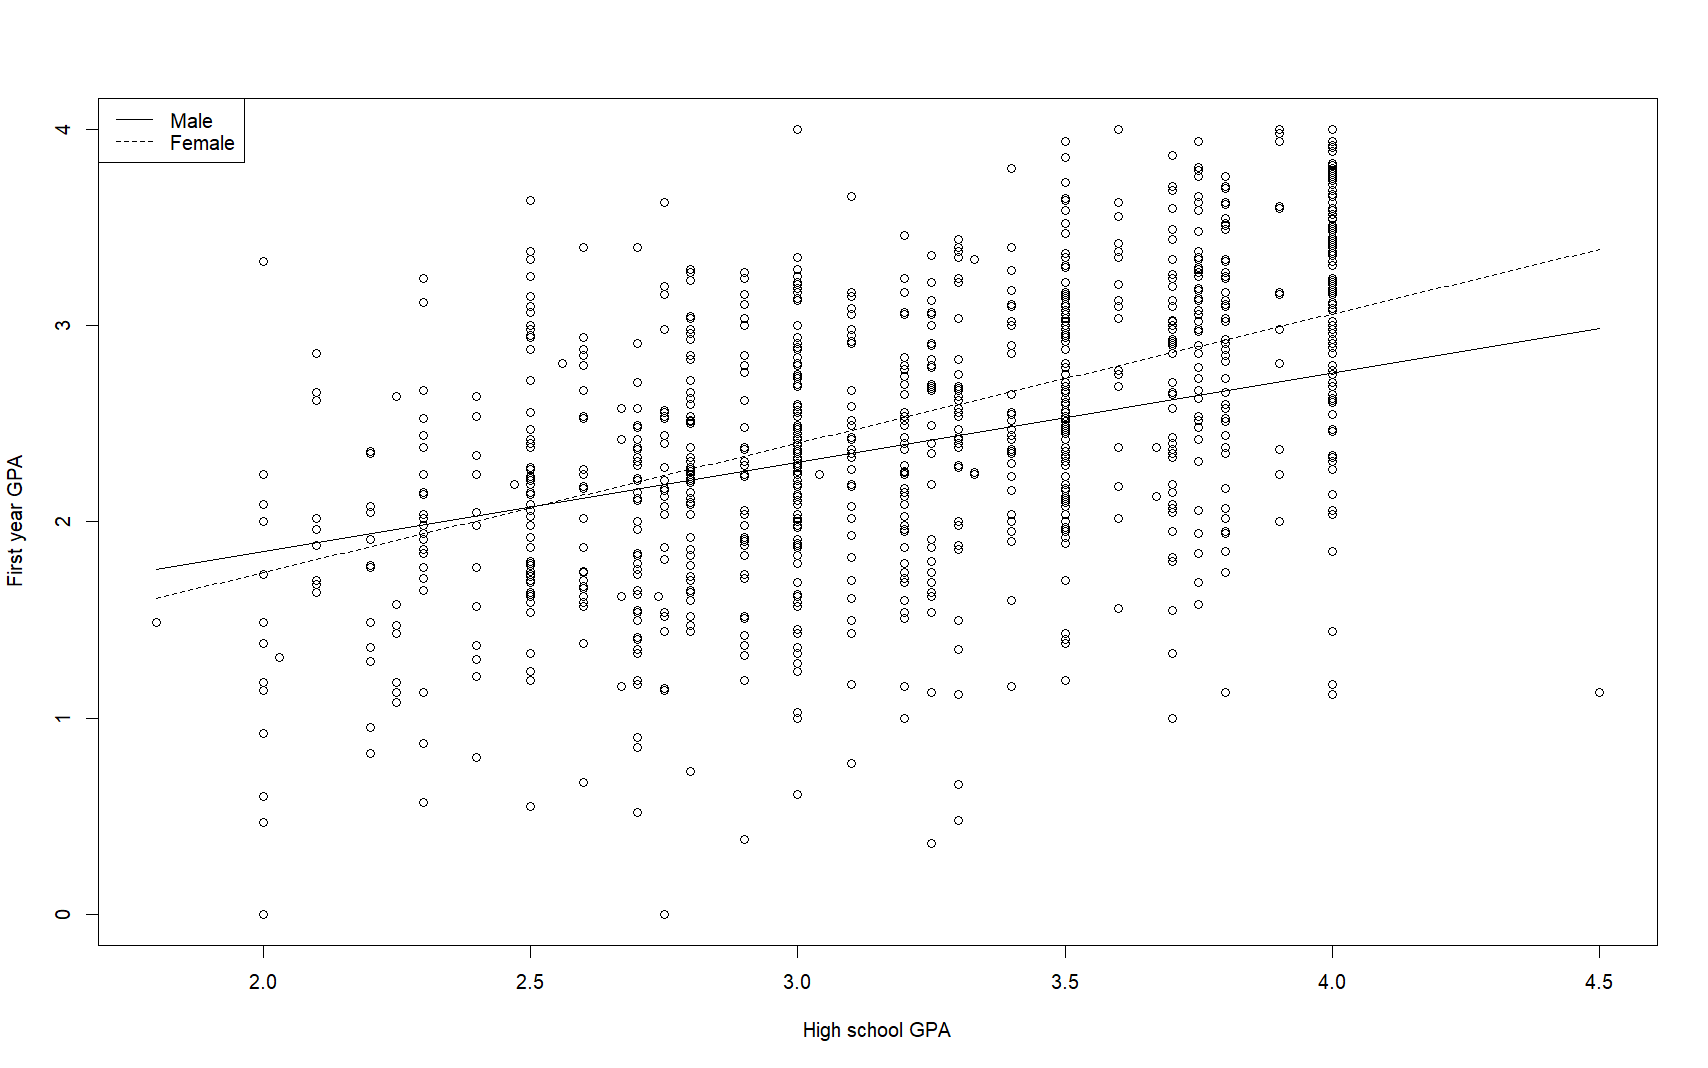
\includegraphics[width=1\linewidth]{Worksheet plots/gpavsgpa.png}
        \caption{High School GPA vs Fitted First Year GPA linear relationship comparison between males and females given fixed SAT Value of satgpa mean.}
\end{figure}
\FloatBarrier
\begin{figure}[h]
    \centering
    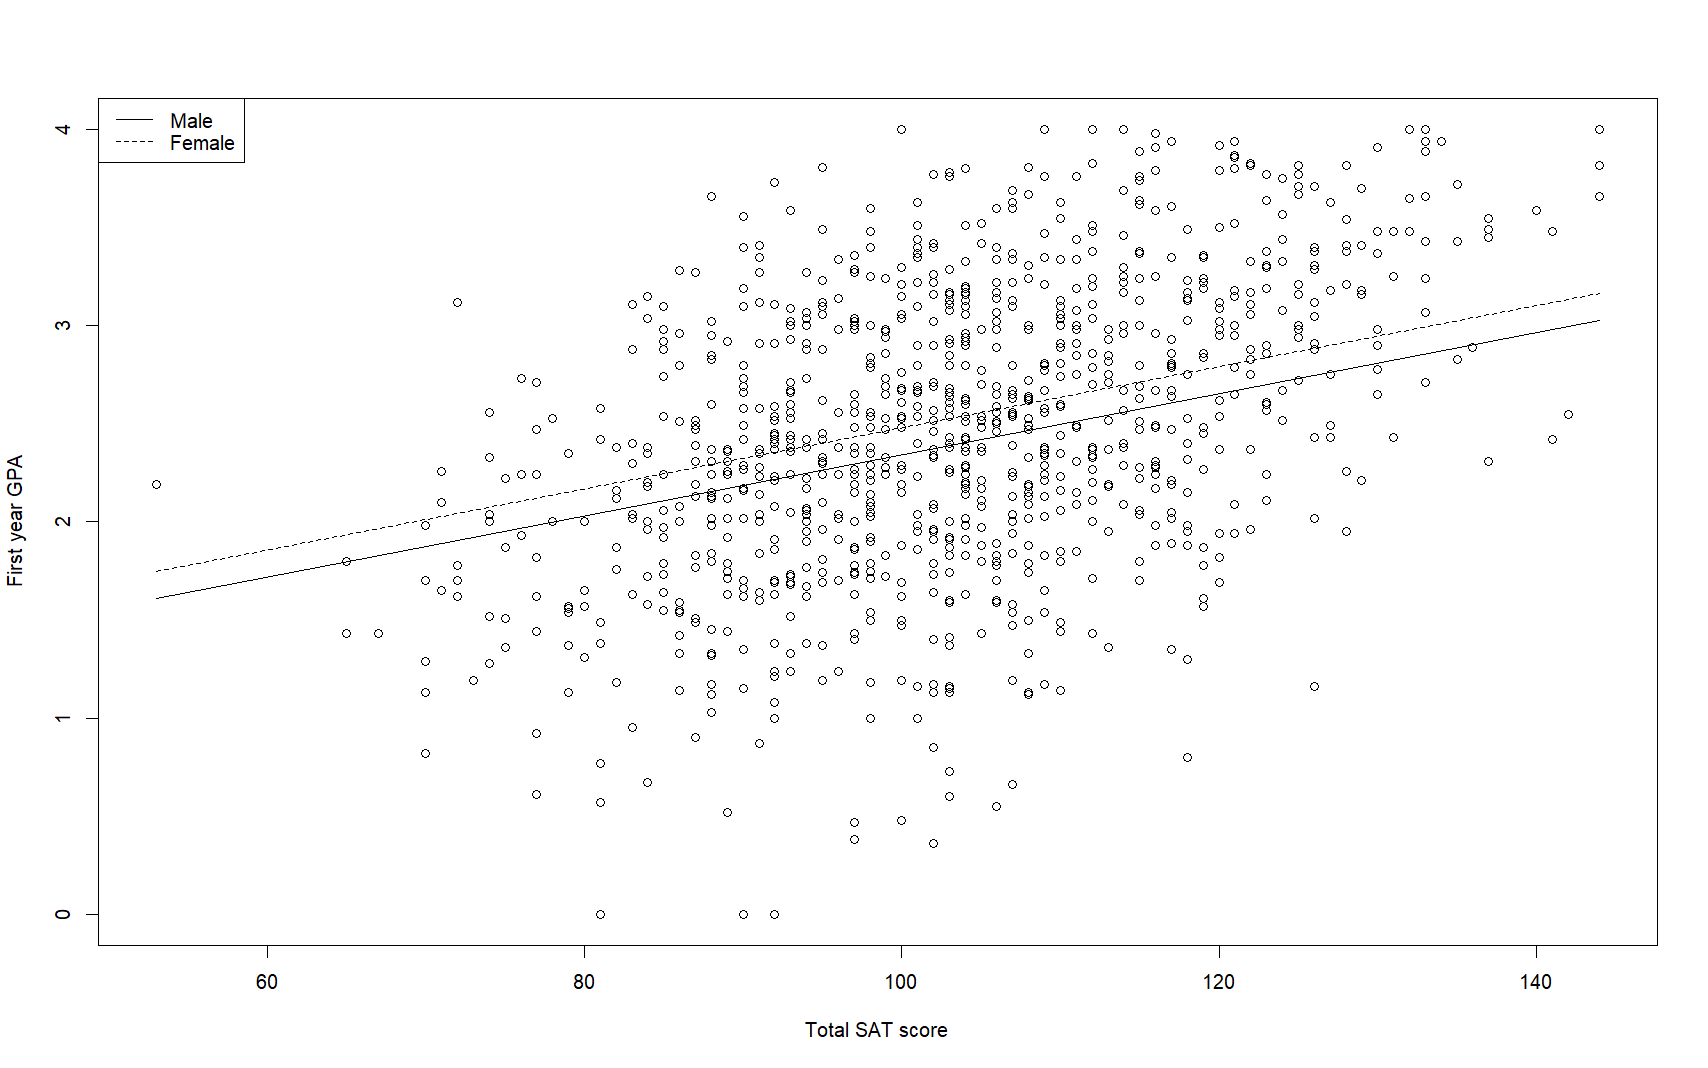
\includegraphics[width=1\linewidth]{Worksheet plots/satvsgpa.png}
    \caption{SAT Score vs First Year GPA linear relationship comparison between males and females given fixed GPA Value of satgpa mean.}
\end{figure}
\FloatBarrier

\noindent Given we have shown $\widehat{\Delta} = -0.508466 + 0.202599 \cdot \textit{hs\_gpa}$, we can observe in Figure 1 that since $\widehat{\Delta} =0 \iff = -0.508466 + 0.202599 \cdot \textit{hs\_gpa} = 0 \implies  \textit{hs\_gpa}\approx2.51$, that is where our straight lines of male and female first year gpas intersect.\newline

\noindent Since $\widehat{\Delta} \perp\!\!\perp \textit{sat\_sum} $, given Figure 2 is based on a fixed value of \textit{hs\_gpa} equal to its mean in satgpa, $\widehat{\Delta}$ is constant which therefore gives us parallel lines in Figure 2.\newline

\noindent From the findings we have made, we can conclude that sex is indeed a factor in influencing students' first year GPA once SAT and high school GPA have been taken into account, and furthermore there is interaction present between sex and high school GPA, which produces non-parallel fitted regression lines for males and females in Figure 1. By contrast, because there is no interaction present between sex and SAT scores, the fitted regression lines in the plot of SAT scores vs first year GPA for males and females are parallel.\newline

\begin{enumerate}
\setcounter{enumi}{4} 
\item Are the model assumptions justifiable given the dataset?
\end{enumerate}



\noindent \textbf{SOLUTION:}\newline

\noindent We will perform a model validation of the model we have determined to provide the best fit to the data:
\begin{lstlisting}[language=R] 
md_hsgpa  <- lm(fy_gpa ~ sat_sum + hs_gpa + factor(sex) + hs_gpa:factor(sex), data = satgpa)\end{lstlisting}

\noindent To do this, we will need to consider whether the standardised residuals are consistent with $\mathcal{N}(0,1)$ and are sufficiently random implying independence. 

\begin{enumerate}
   \item   \noindent We firstly notice from the following \textsf{R} code that approximately $95\%$ of the standardised residuals lie in the interval $(-2,2)$ which is roughly what we would expect under $\mathcal{N}(0,1)$. 
    \begin{lstlisting}[language=R]
> stdres <- rstandard(md_hsgpa)
> proportion_abs_stdres_less_2 <- mean(abs(stdres) <= 2)  
> proportion_abs_stdres_less_2
[1] 0.952     \end{lstlisting}

    \item \noindent We can now assess whether the residuals plotted against their index number generated by the following \textsf{R} code display any form of pattern (e.g. funnelling) which could indicate a lack of independence.
    \begin{lstlisting}[language=R]
plot(stdres,xlab = "Index",ylab = "Standardised residuals", main = "satgpa data indices vs standardised residuals")
abline(h = 0)   \end{lstlisting}

    \begin{figure}[h]
        \centering
        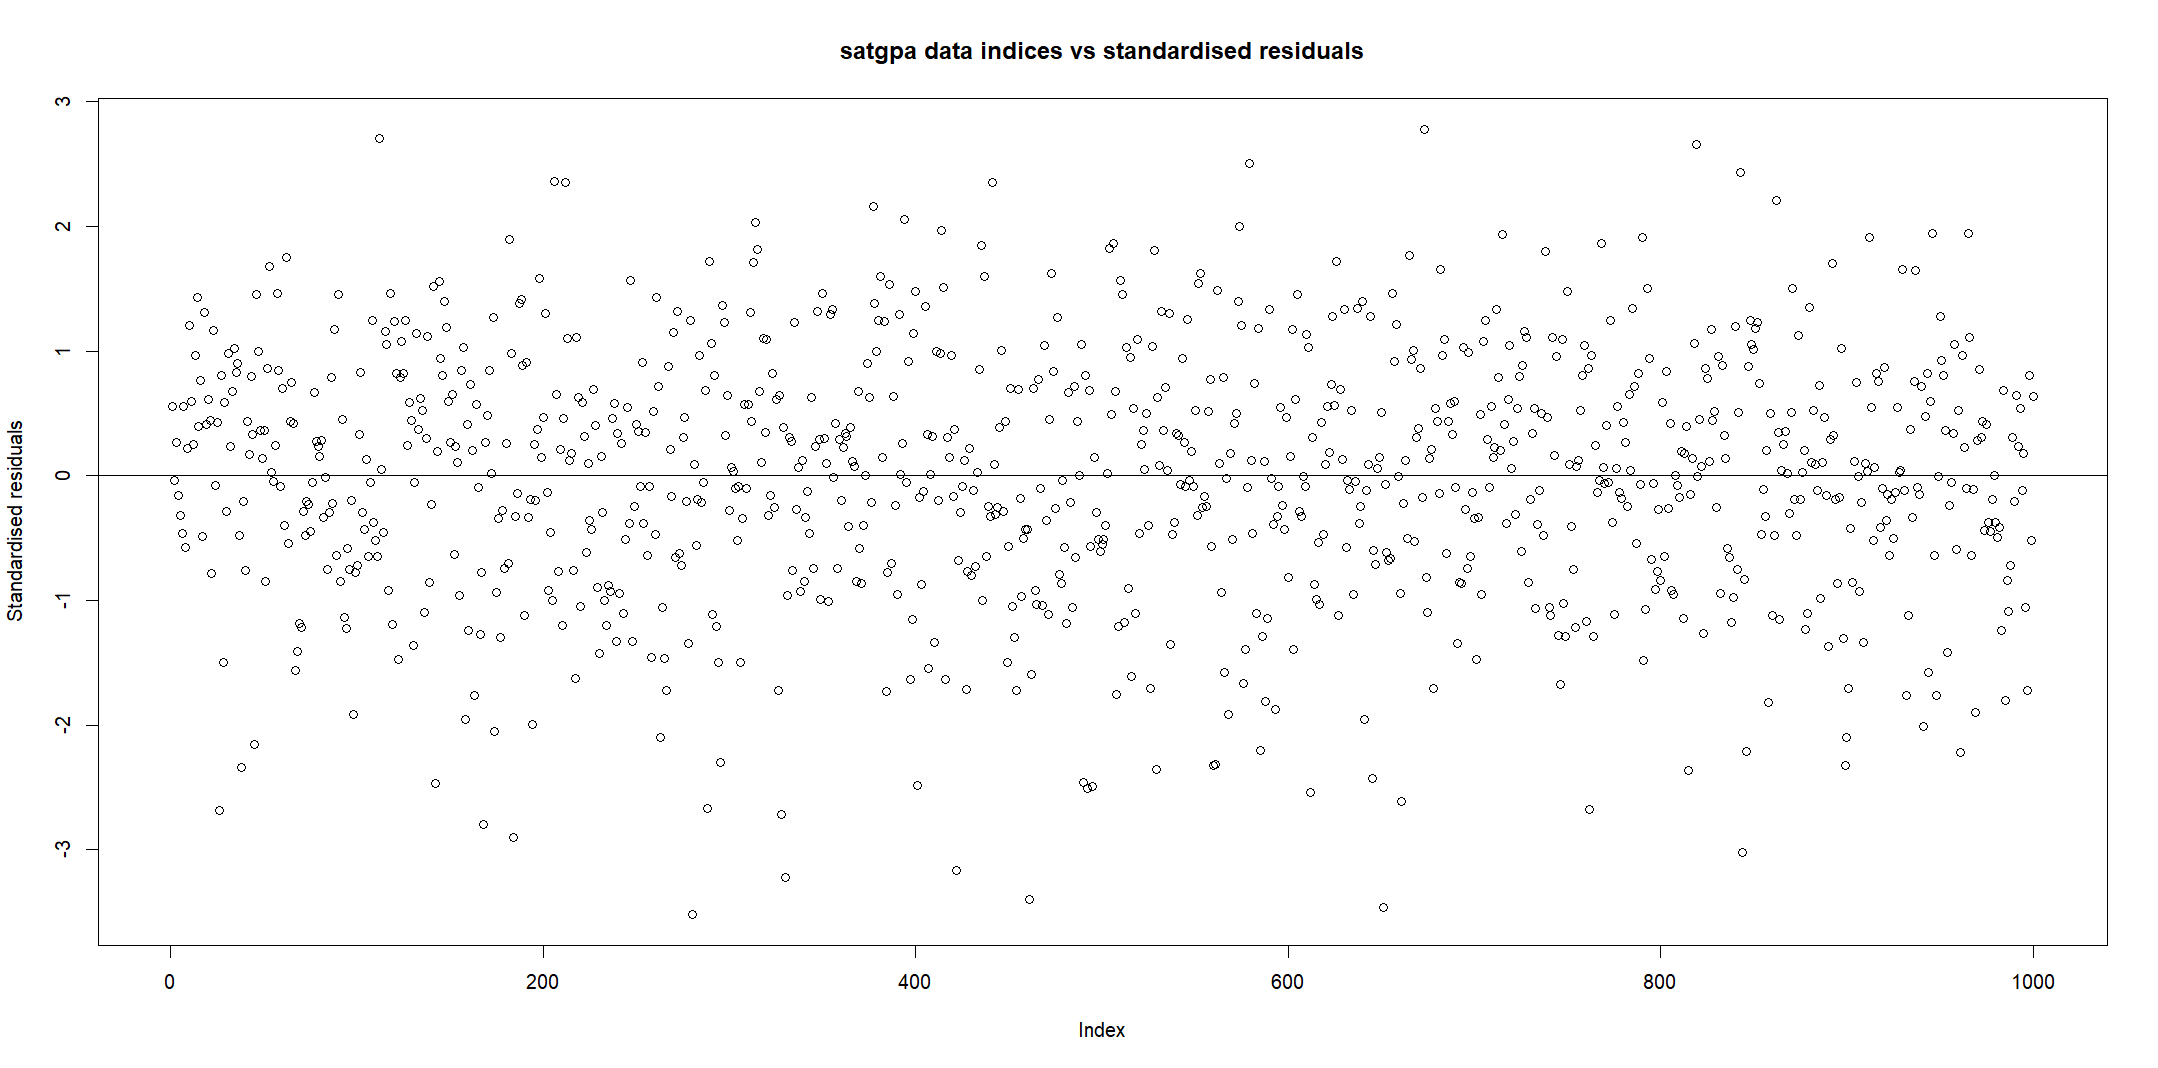
\includegraphics[width=1\linewidth]{Worksheet plots/index_resid.png}
        \caption{satgpa data indices vs standardised residuals}
    \end{figure}\FloatBarrier

    \noindent Figure 3 demonstrates that the standardised residuals plotted against their indices are randomly scattered about zero with no apparent patterns, hence the assumption of error independence seems to be upheld.


    \item \noindent We can now assess whether the residuals demonstrate constant variance by plotting them against each regressor and the fitted values. Each plot is accompanied by its corresponding block of \textsf{R} code.

    \noindent Standardised residuals vs \textit{sat\_sum}:
    \begin{lstlisting}[language=R]
plot(satgpa$sat_sum, stdres,xlab = "satgpa$sat_sum",ylab = "Standardised residuals",main = "SAT Totals vs Standardised Residuals")
abline(h = 0)     \end{lstlisting}

    \begin{figure}[h]
        \centering
        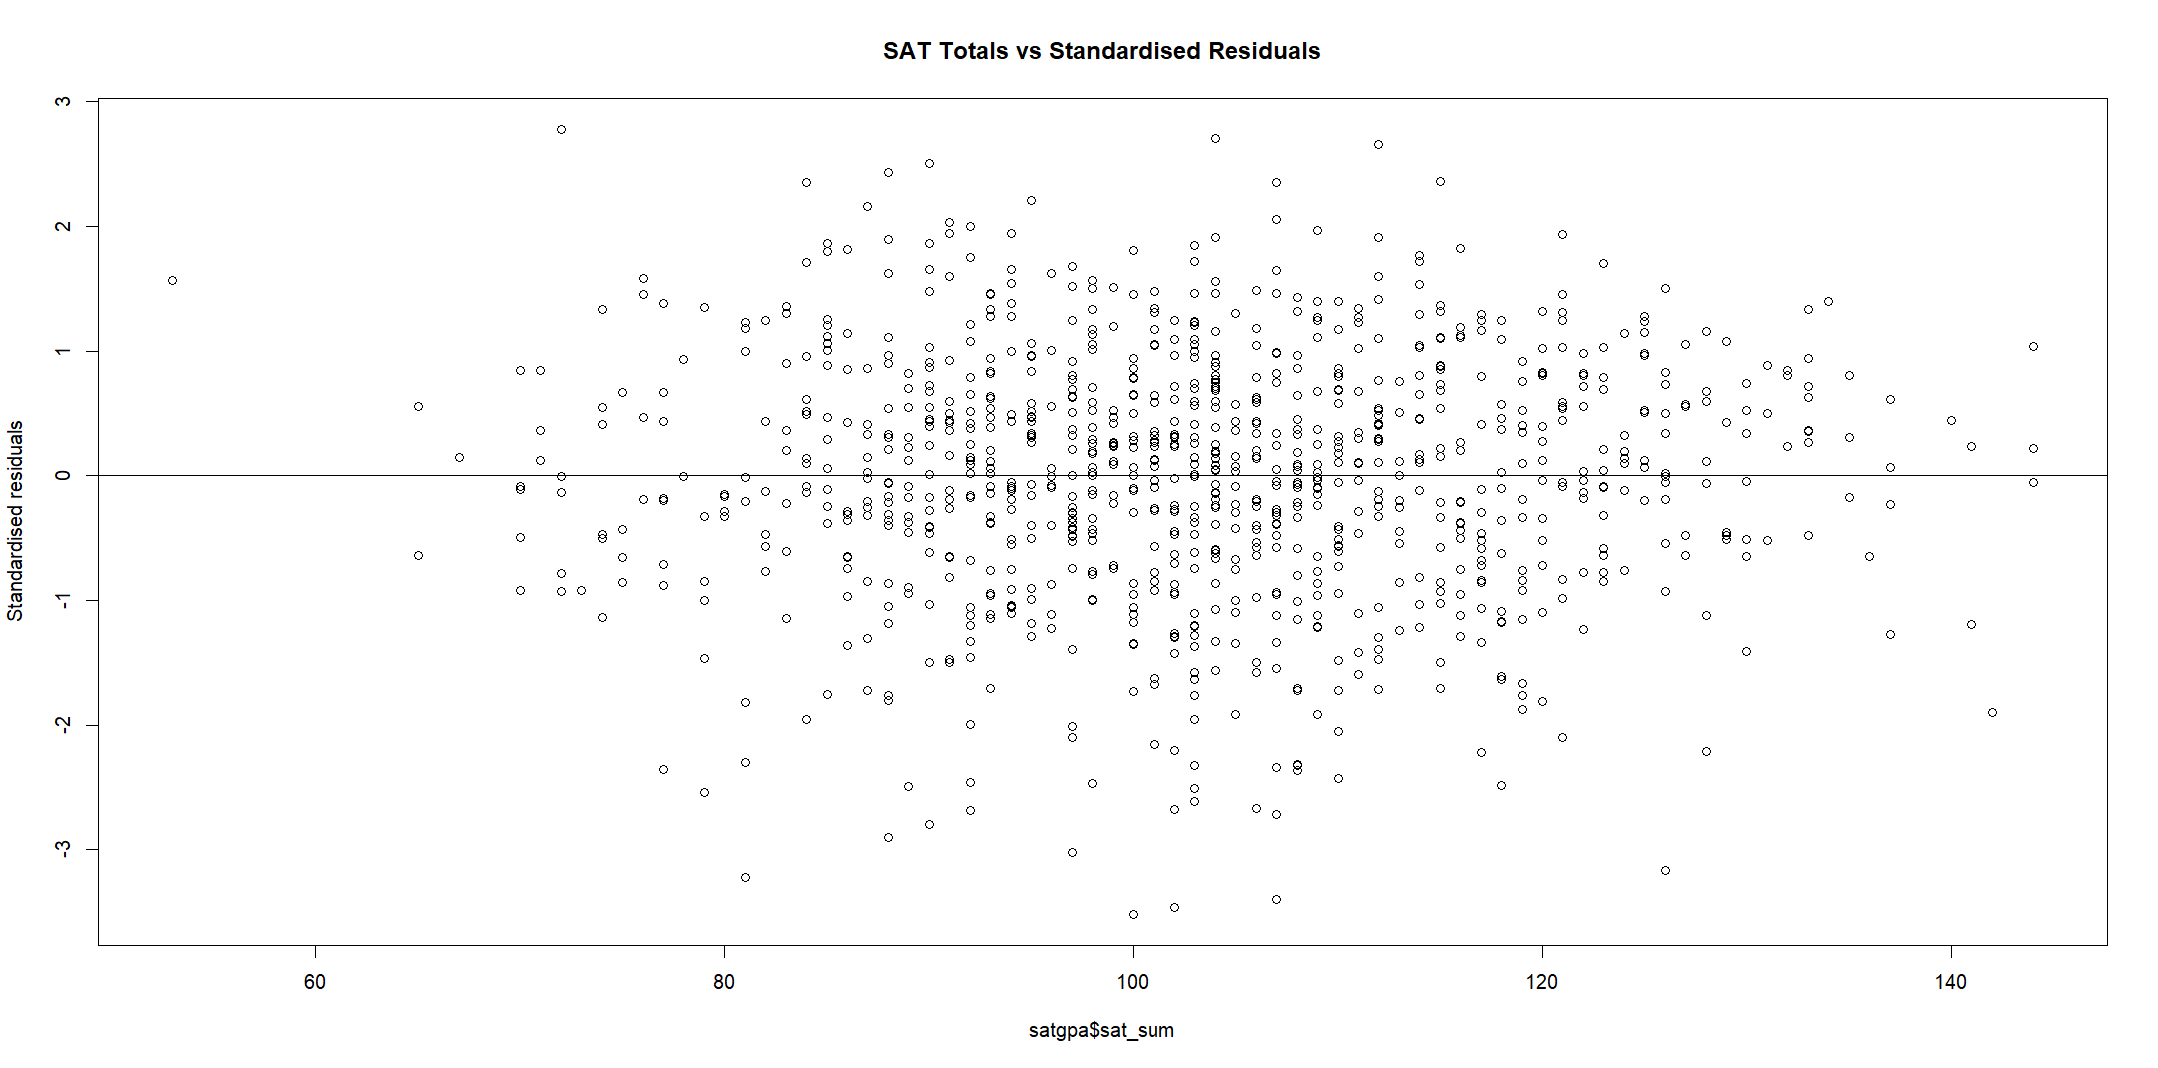
\includegraphics[width=1\linewidth]{Worksheet plots/resid_vs_satsum.png}
        \caption{SAT Totals vs Standardised Residuals}
    \end{figure}\FloatBarrier

    \noindent Standardised residuals vs \textit{hs\_gpa}:
    \begin{lstlisting}[language=R]
plot(satgpa$hs_gpa, stdres,xlab = "satgpa$hs_gpa",ylab = "Standardised residuals",main = "High School GPA vs Standardised Residuals")
abline(h = 0)    \end{lstlisting}

    \begin{figure}[h]
        \centering
        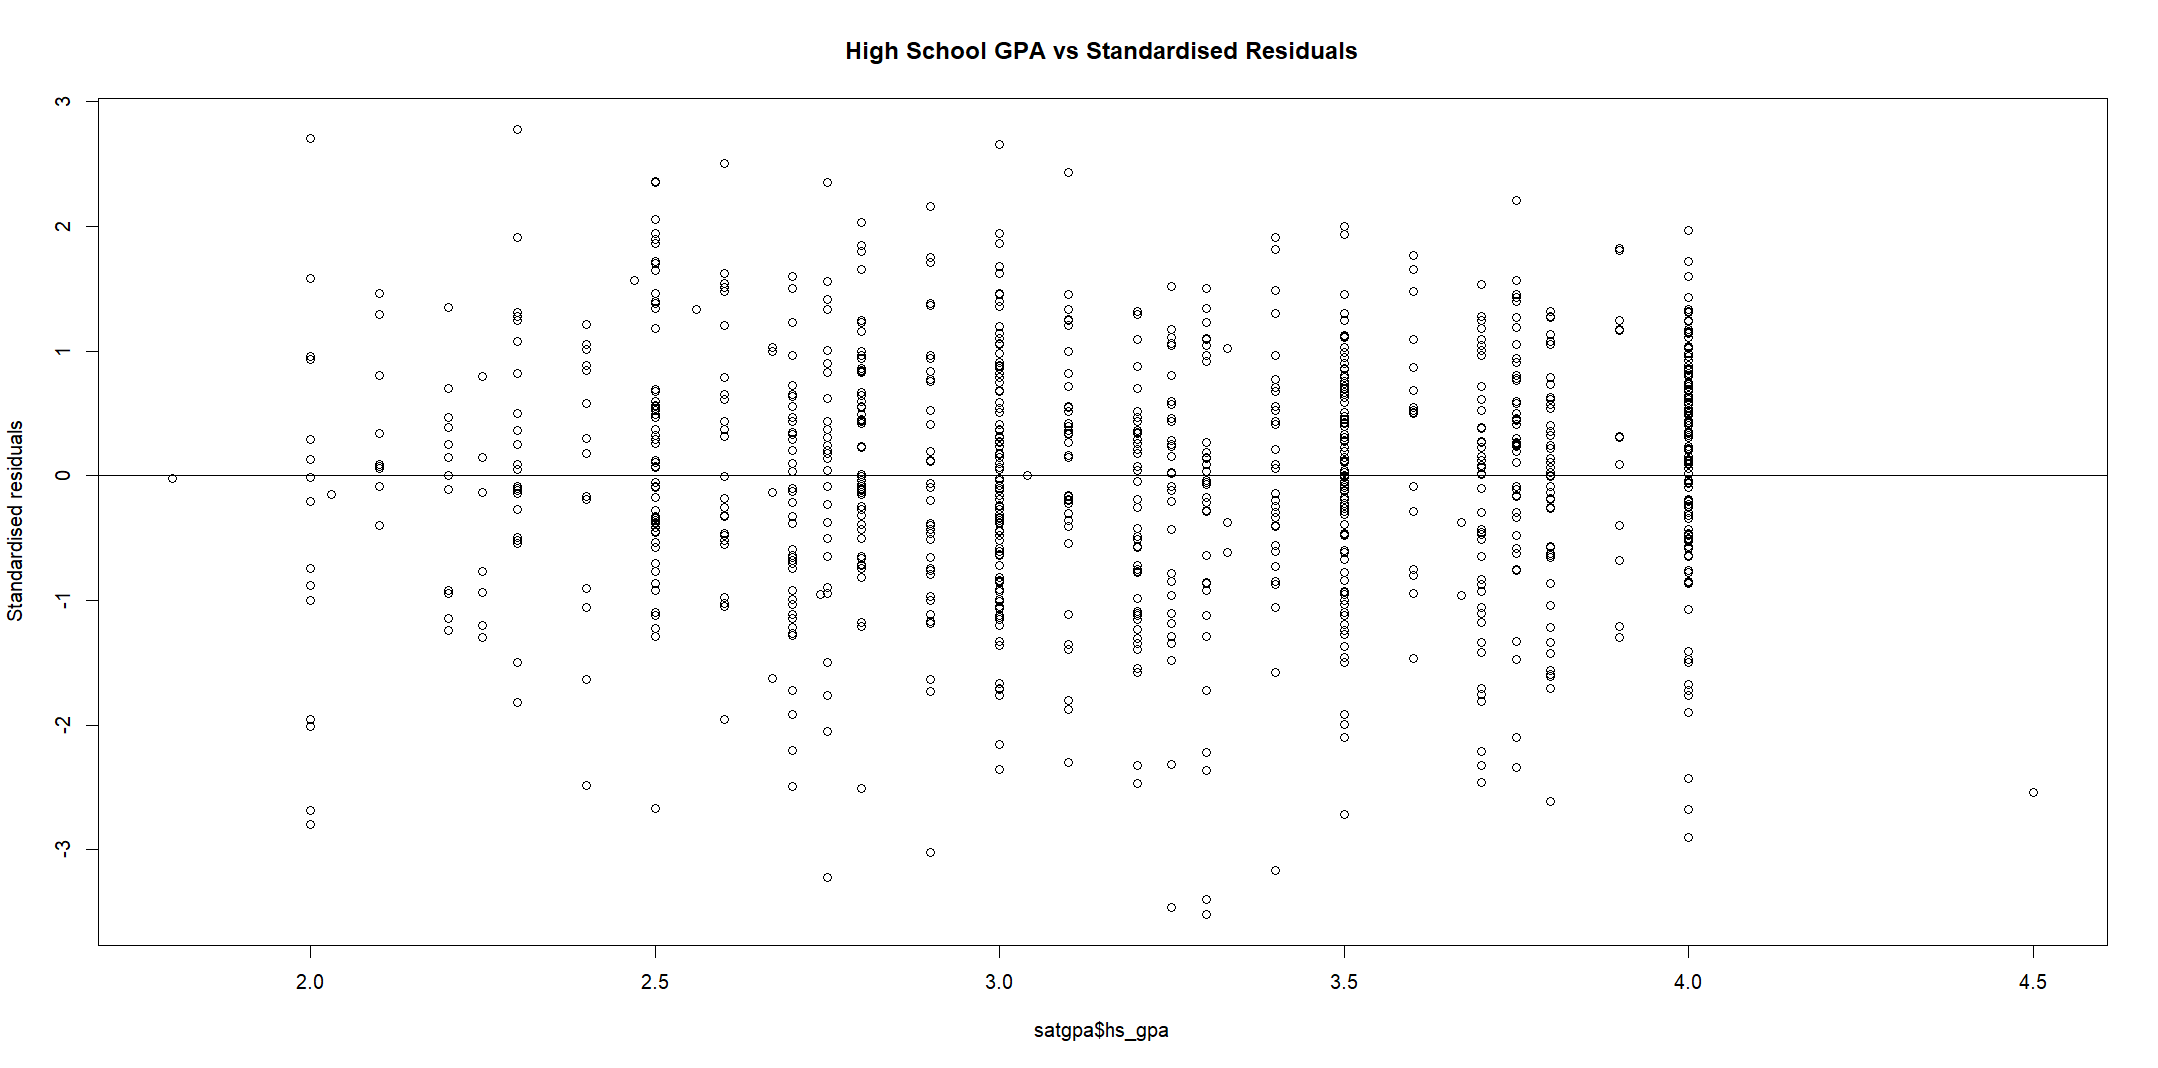
\includegraphics[width=1\linewidth]{Worksheet plots/resid_vs_hsgpa.png}
        \caption{High School GPA vs Standardised Residuals.}
    \end{figure}\FloatBarrier

    \noindent Standardised residuals vs fitted values:
    \begin{lstlisting}[language=R]
plot(md_hsgpa$fitted.values, stdres, xlab = "md_hsgpa$fitted.values", ylab ="Standardised residuals",main = "Model fitted values vs Standardised Residuals")
abline(h = 0)   \end{lstlisting}

    \begin{figure}[h]
        \centering
        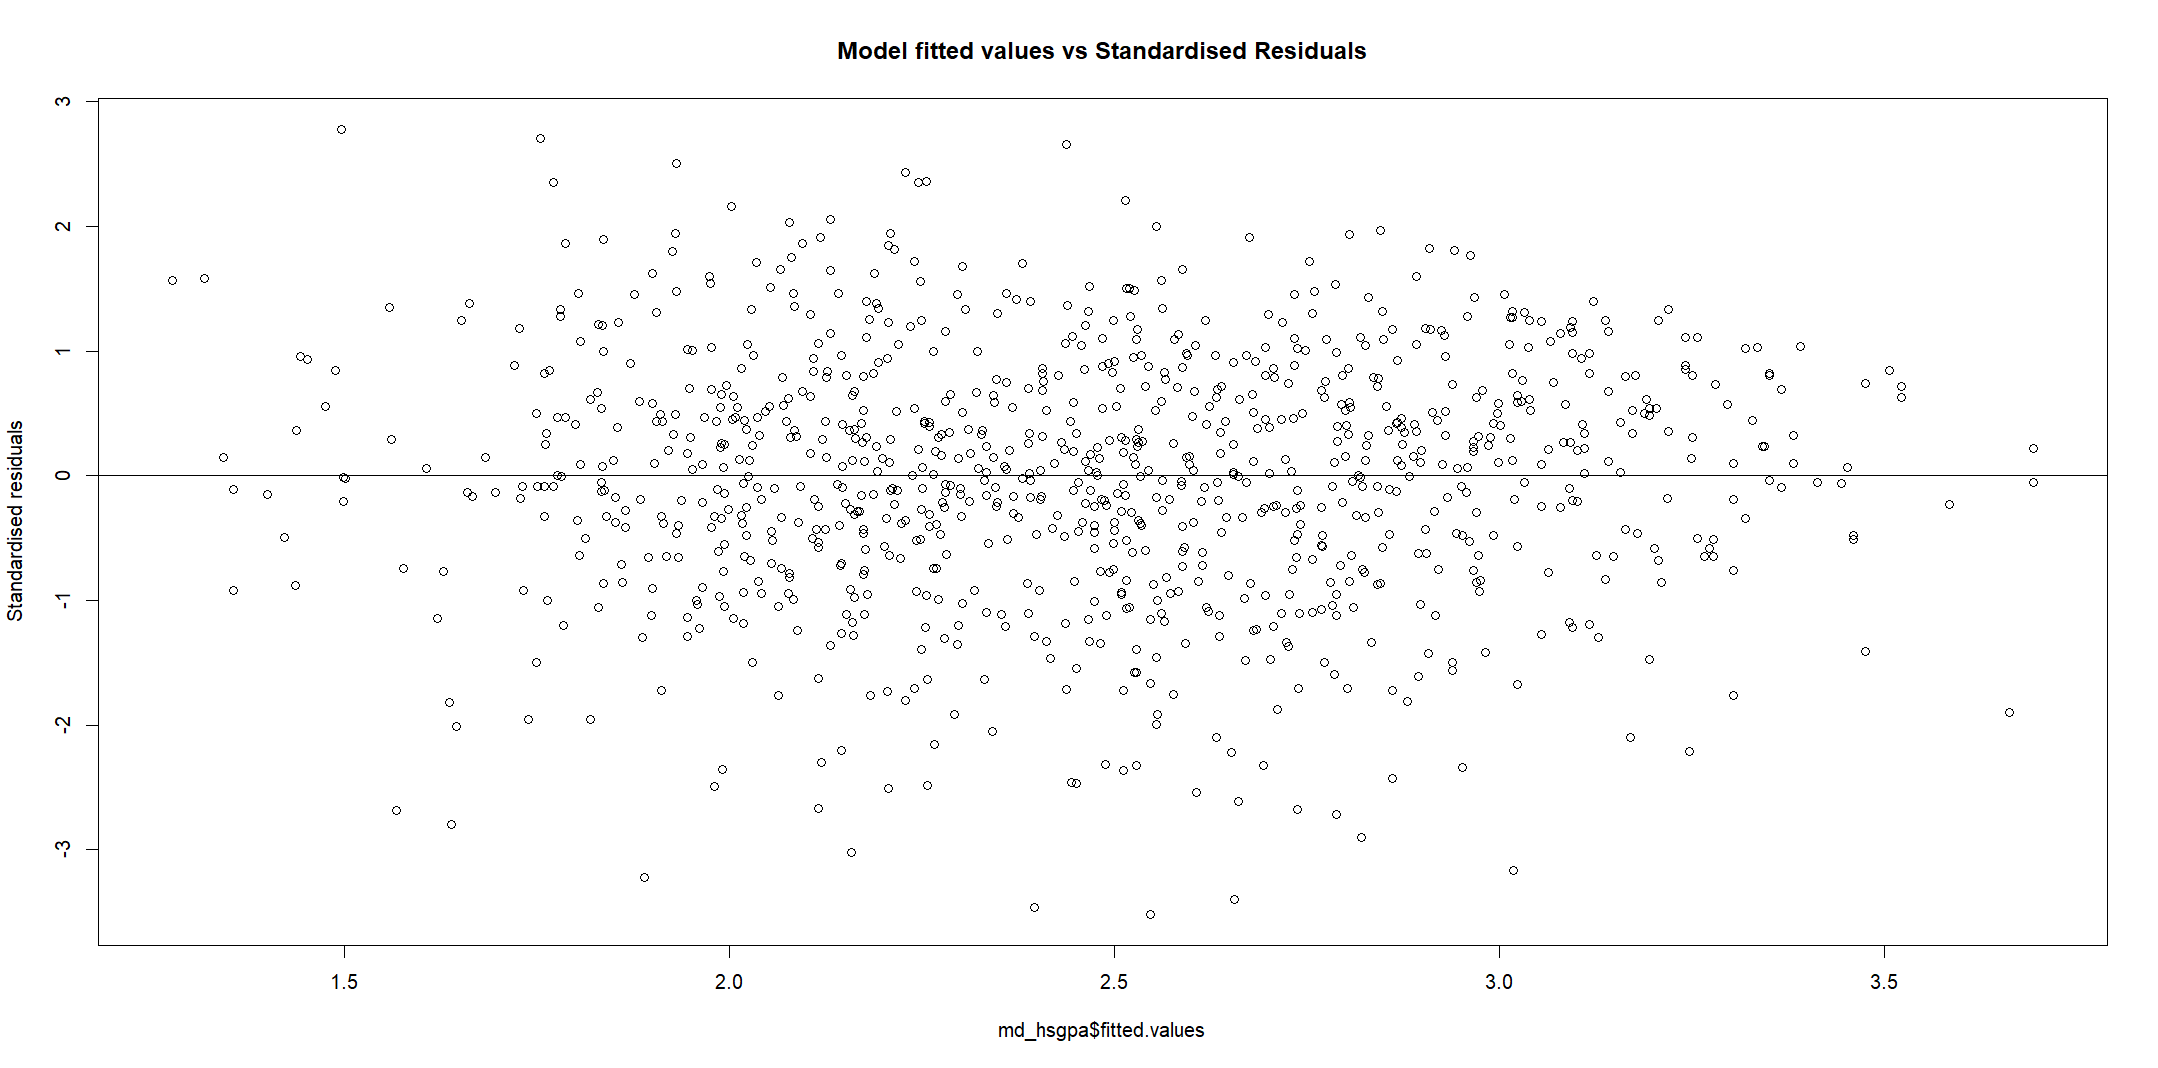
\includegraphics[width=1\linewidth]{Worksheet plots/resid_vs_fitted.png}
        \caption{Model fitted values vs Standardised Residuals}
    \end{figure}\FloatBarrier

    \noindent Figures 4,5,6 demonstrate even spread of standardised residuals about zero within a fairly uniform band since as we showed, most values fall within the interval $(-2,2)$. Since there does not seem to be any pattern to the distribution or change in vertical spread of the standardised residuals in any of these plots, we can conclude that the assumption of constant error variance is upheld.


\item    \noindent We now want to confirm the normality assumption by producing a Normal Probability (QQ) plot and a histogram of the standardised residuals in \textsf{R}:
    \begin{lstlisting}[language=R]
qqnorm(stdres, main = "Normal QQ plot")
qqline(stdres)

hist(stdres,30,xlab = "Standardised residuals",main = "Histogram of standardised residuals")    \end{lstlisting}

    \begin{figure}[h]
        \centering
        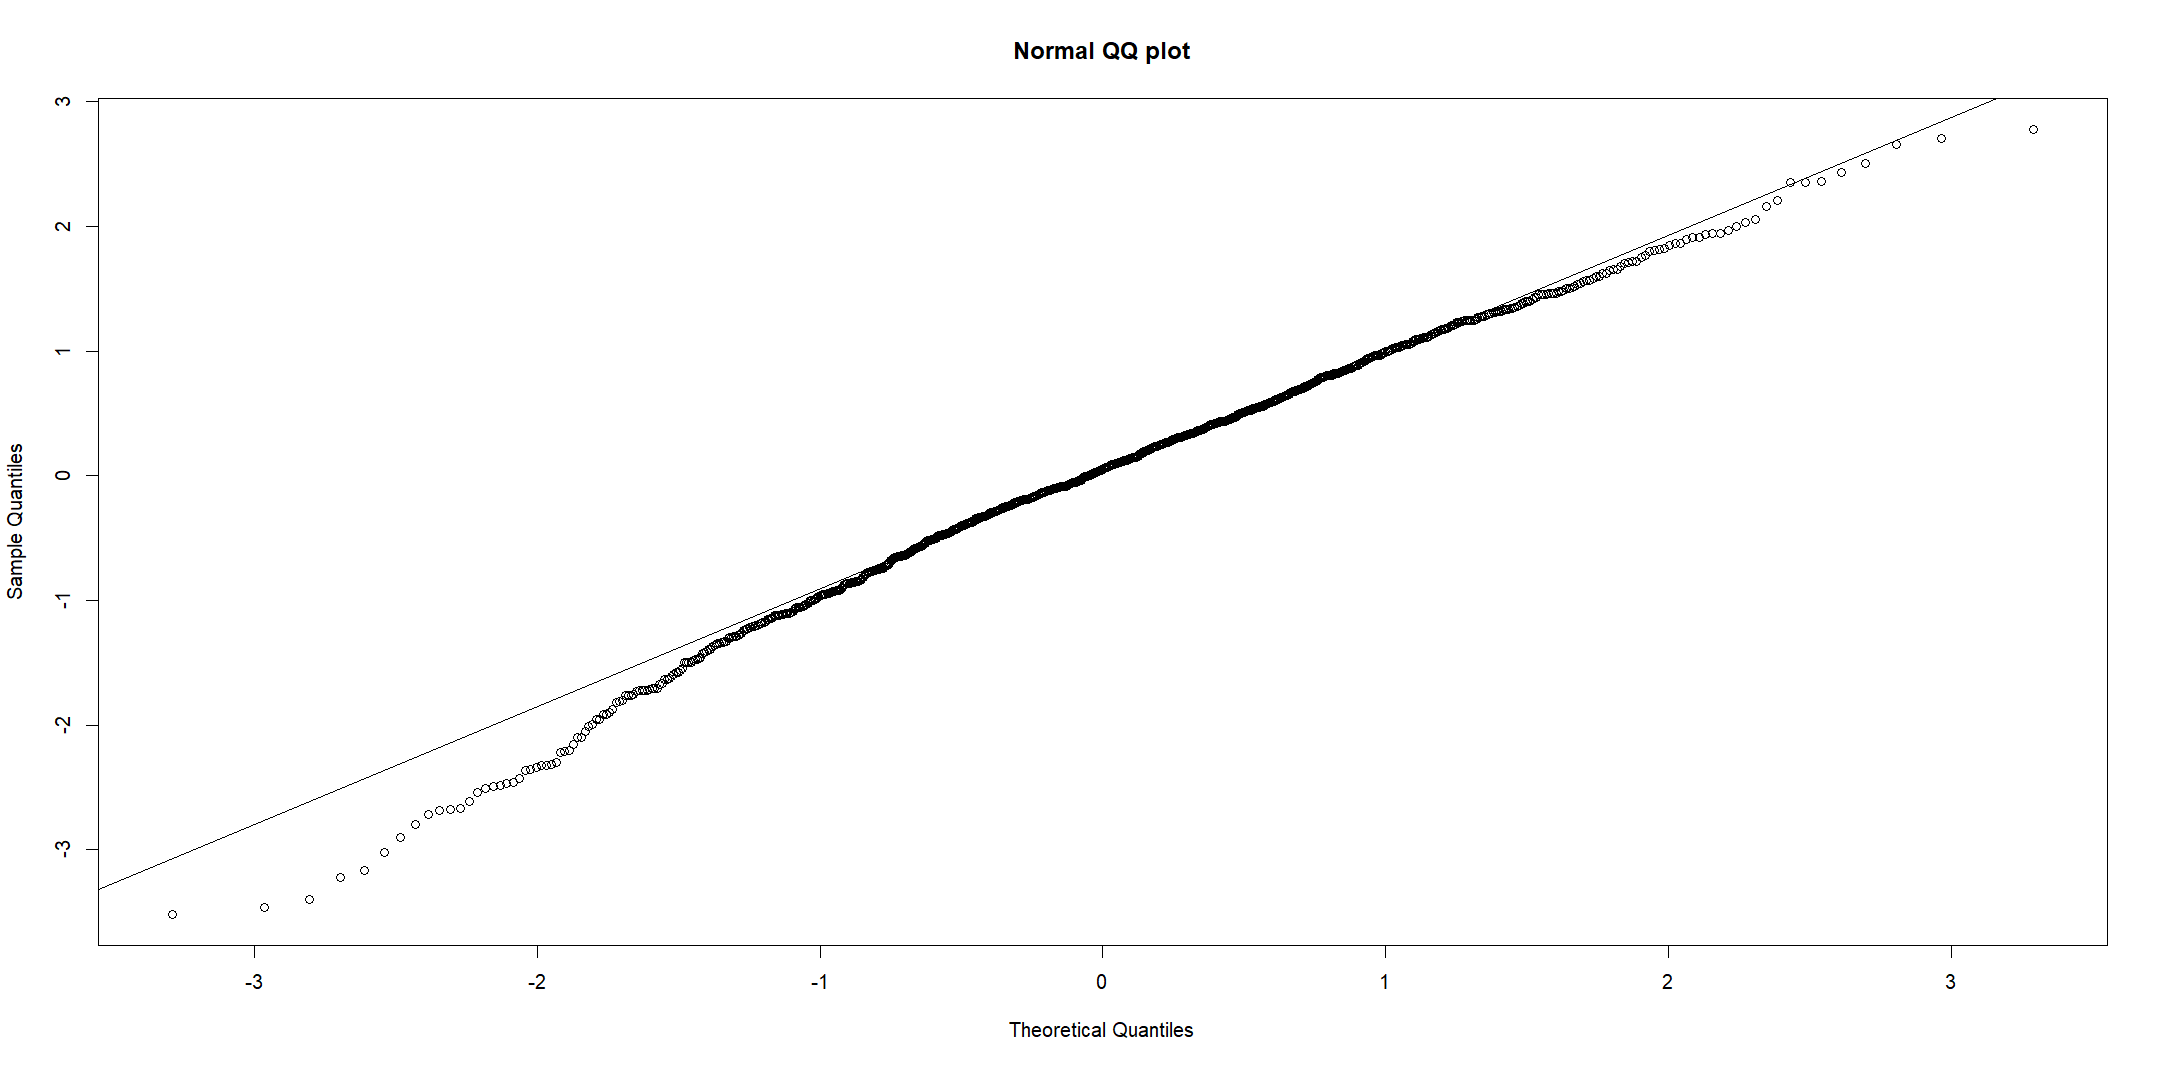
\includegraphics[width=1\linewidth]{Worksheet plots/qqplot_resid.png}
        \caption{Normal QQ plot.}
    \end{figure}\FloatBarrier

    \begin{figure}[h]
        \centering
        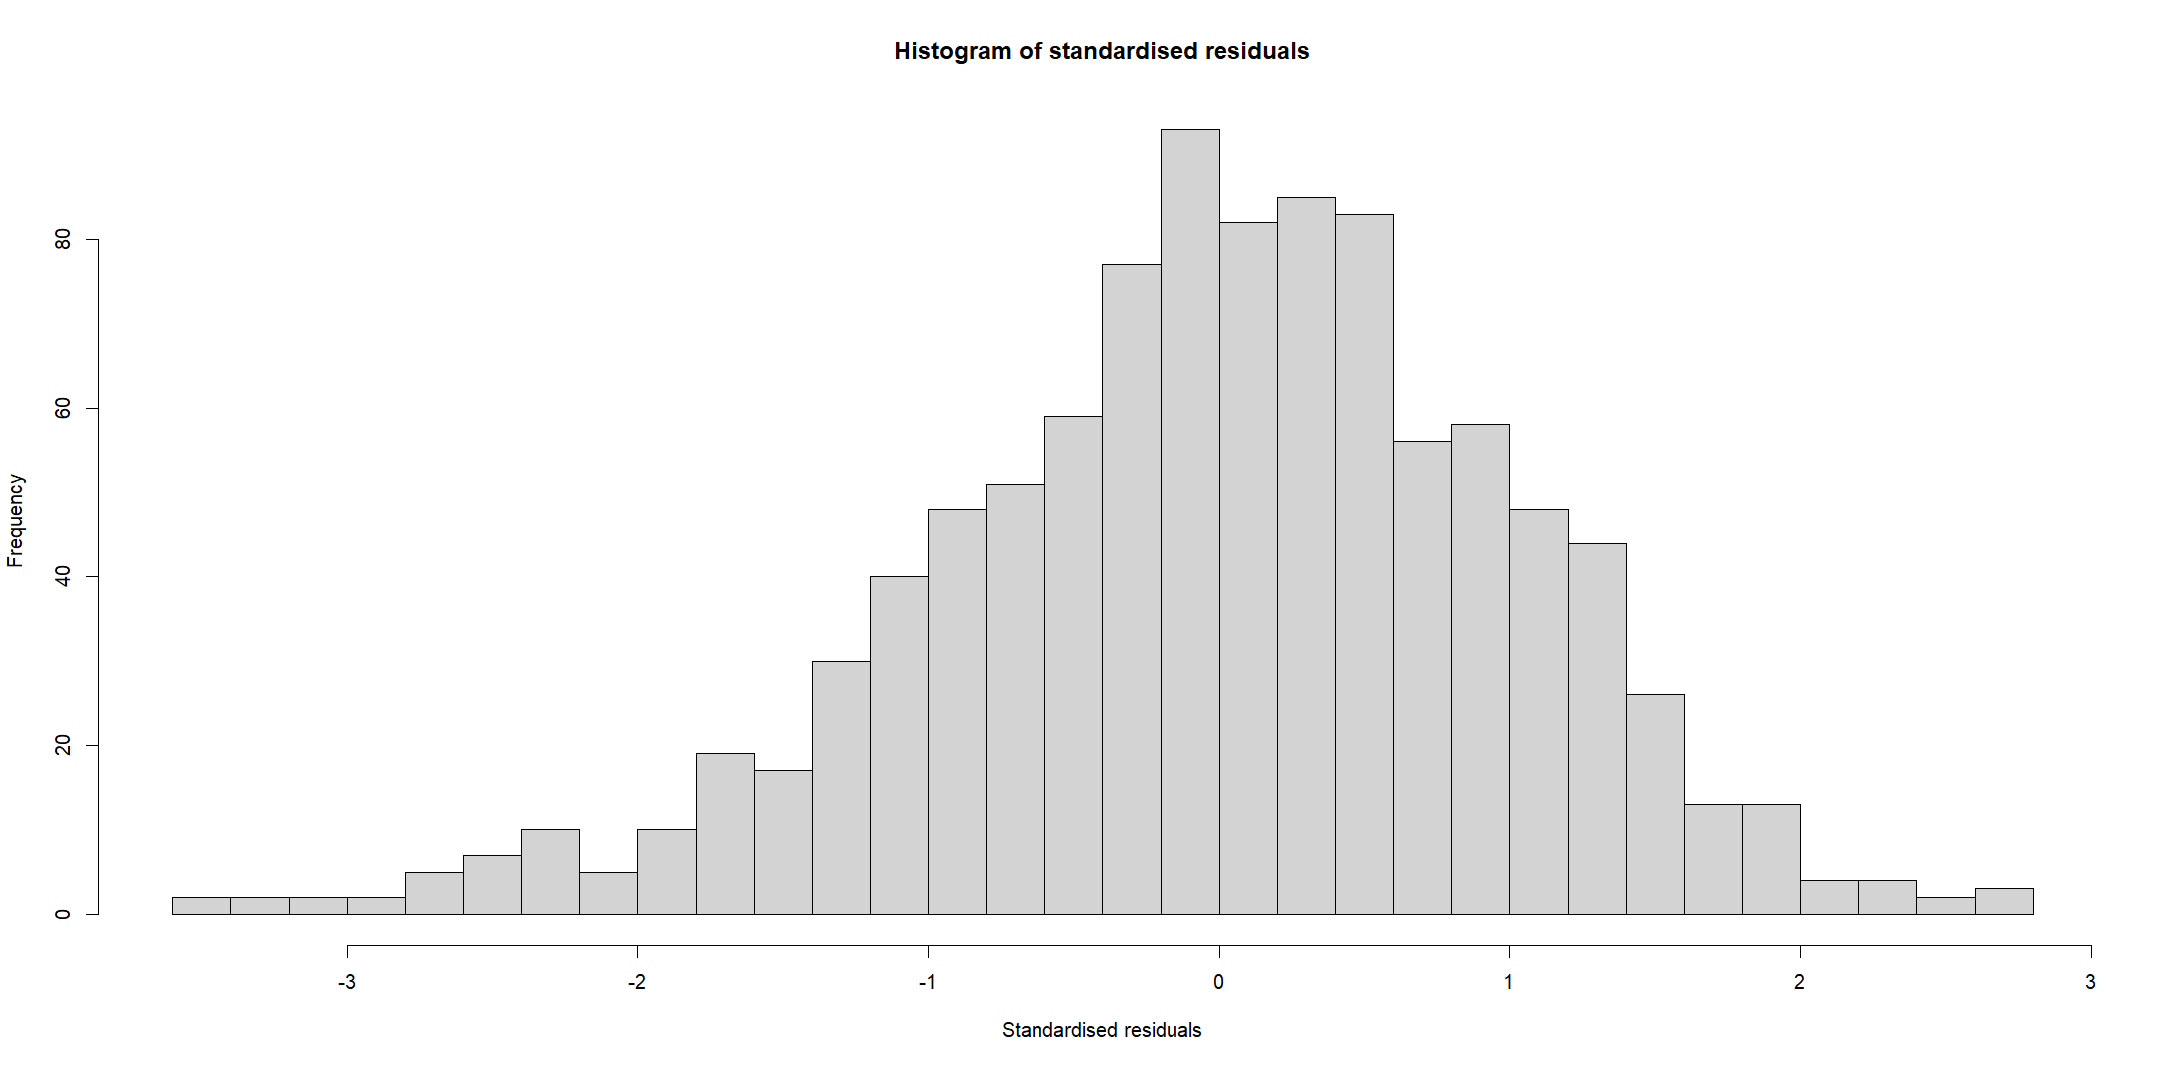
\includegraphics[width=1\linewidth]{Worksheet plots/hist_resid.png}
        \caption{Histogram of standardised residuals.}
    \end{figure}\FloatBarrier

    \noindent We observe in Figure 7 that the points on the QQ plot all seem to lie on, or close to the straight line, with only minor deviations in the tails near $-1.5$ and $2$. Then in Figure 8 we observe that the histogram is both roughly symmetric and bell-shaped. Since we have confirmed that approximately $95\%$ of the standardised residuals lie in the interval $(-2,2)$, this provides strong support of the assumption that they follow $\mathcal{N}(0,1)$.

    \item    \noindent Finally, we want to consider whether the error variance is constant between the two levels of the sex factor using a boxplot of standardised residuals by sex:
    \begin{lstlisting}[language=R]
boxplot(stdres ~ factor(sex), data = satgpa, xlab = "Sex : 1 = Male, 2 = Female", ylab= "Standardised residuals", main = "Boxplot of Sex vs Standardised residuals")\end{lstlisting}

    \begin{figure}[h]
        \centering
        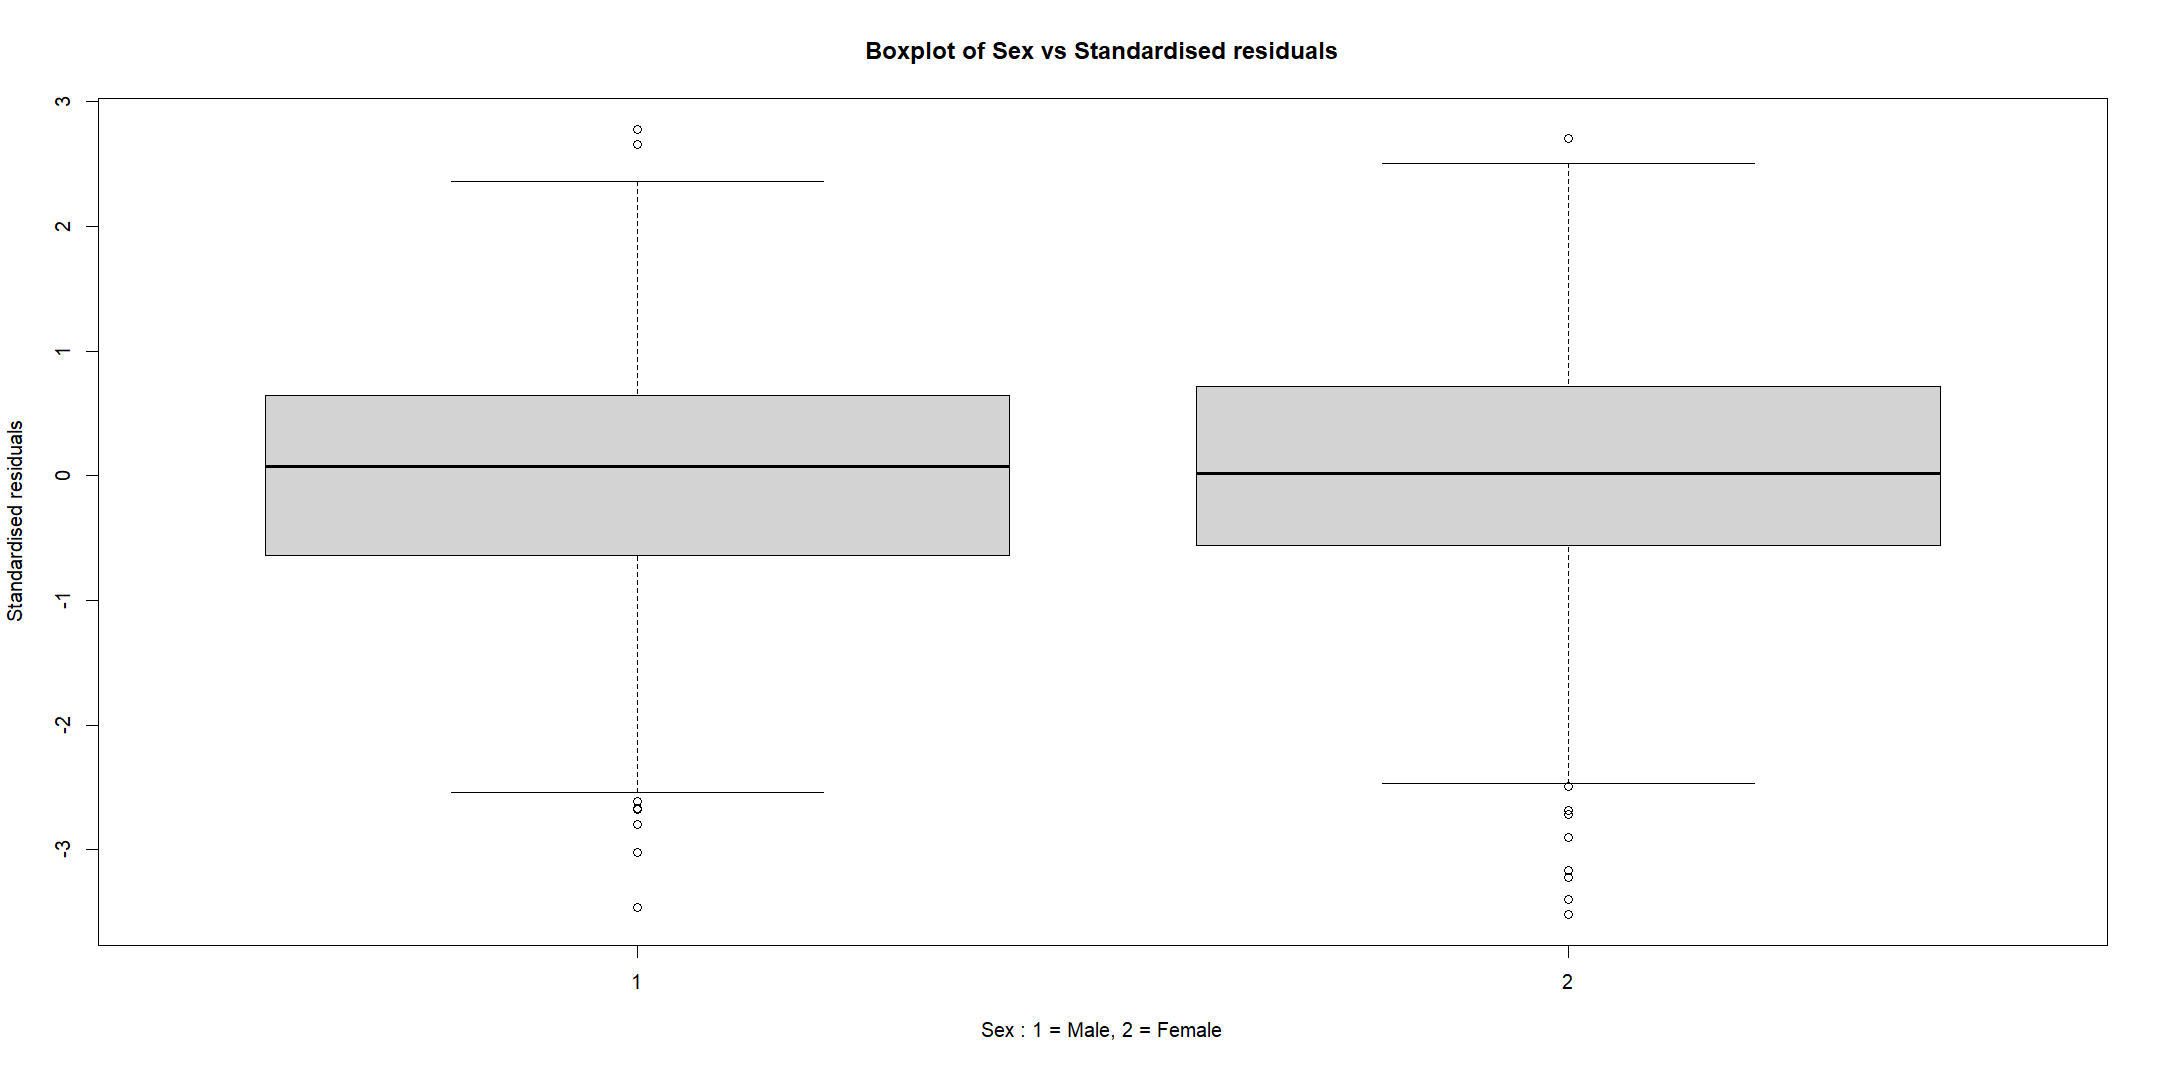
\includegraphics[width=1\linewidth]{Worksheet plots/resid_by_sex.png}
        \caption{Boxplot of Sex vs Standardised residuals}
    \end{figure}\FloatBarrier

    \noindent We can see in Figure 9 that both levels of the factor sex have medians very close to zero, and similar interquartile ranges and variance. This supports the assumption of constant variance in standardised residuals across both levels of the qualitative factor sex in our model.

\end{enumerate}


\noindent In conclusion, the standardised residuals appear to be consistent with a Normal distribution with mean zero and constant variance, i.e.\ $\mathcal{N}(0,1)$. Given that approximately $95\%$ lie in the interval $(-2,2)$, the residual plots show a random scatter of points with no clear patterns in the data, and the QQ plot and histogram are roughly aligned with what we expect under Normality (points close to a straight line in the QQ plot and an approximately bell-shaped histogram). We also see no evidence of change in variance in any of the residual plots, either for the quantitative regressors or across the levels of the qualitative regressor. Therefore, for the model we proposed, the relevant assumptions appear to be upheld.


\hrulefill
\end{document}
